\documentclass[nocc]{template/openetcs_report}
% Use the option "nocc" if the document is not licensed under Creative Commons
%\documentclass[nocc]{template/openetcs_report}
\usepackage{lipsum,url}
\usepackage{supertabular}
\usepackage{multirow}
\usepackage{color, colortbl}
\definecolor{gray}{rgb}{0.8,0.8,0.8}
\usepackage[modulo]{lineno}
\graphicspath{{./template/}{.}{./images/}}
\begin{document}
\frontmatter
\project{openETCS}

%Please do not change anything above this line
%============================
% The document metadata is defined below

%assign a report number here
\reportnum{OETCS/WP5/M5.1}

%define your workpackage or task here
\wp{openETCS@ITEA Work-Package 5: ``Demonstrator''}

%set a title here
\title{EVC simulator architecture}

%set a subtitle here
%\subtitle{The introduction of openETCS's \LaTeX class, Version~1.1}

%set the date of the report here
\date{June 2014}

%document approval
%define the name and affiliation of the people involved in the documents approbation here
\creatorname{Alexis Julin}
\creatoraffil{ERSA}

\techassessorname{Nicolas Van Landeghem}
\techassessoraffil{ERSA}

\qualityassessorname{Ainhoa Gracia}
\qualityassessoraffil{SQS}

\approvalname{Klaus-R\"udiger Hase}
\approvalaffil{DB Netz}

%define a list of authors and their affiliation here
\author{Eric Schellenberg, Nicolas Van Landeghem, Didier Weckmann, Alexis Julin}
\affiliation{ERSA\\
5 Rue Maurice Blin \\
67500 Haguenau, France}

% define the coverart
\coverart[width=350pt]{openETCS_EUPL.png}

%define the type of report
\reporttype{Final Report}


\begin{abstract}
%define an abstract here
The purpose of this document is to describe the architecture of the EVC simulator: its breakdown into modules, the exchanged data, and the interfaces with external devices.
The EVC simulator behaves according to the SRS Class 1 version 3.3.0.
The first part of this document describes the context of the EVC simulator, its interfaces and its breakdown into modules.
The following parts describe for each modules of the ERSA EVC simulator the exchanged data, the allocated functions.
\end{abstract}

%=============================
%Do not change the next three lines
\maketitle

%Modification history
%if you do not need a modification history table for your document simply comment out the eight lines below
%=============================
\section*{Modification History}
\tablefirsthead{
\hline
\rowcolor{gray}
Version & Section & Modification / Description & Author \\\hline}
\begin{supertabular}{| m{1.2cm} | m{1.2cm} | m{6.6cm} | m{4cm} |}
 0.1&All parts &Creation &Eric Schellenberg \\\hline
 1.0&All parts &Official version &Eric Schellenberg \\\hline
 1.1&All parts &Update &Eric Schellenberg \\\hline
 2.0&All parts &Update for OpenETCS review &Alexis Julin \\\hline
\end{supertabular}

\tableofcontents
\listoffiguresandtables

%=============================
%Uncomment the next line if you need line numbers for tracebility when the document is in review
%\linenumbers

%=============================
% The actual document starts below this line
%=============================

%Start here
\mainmatter
\chapter{Introduction}
\section{Overview of European Vital Computer (EVC)}
The European Vital Computer (EVC) is the brain or kernel of the ERTMS/ETCS system which is installed in trains. It allows the safe movement of trains on lines equipped with ERTMS/ETCS. It uses a certain number of interfaces with other equipments. Some of them are defined as mandatory at FFFIS or FIS level, and some others are not standard.
\begin{figure}[!h]
  \centering
  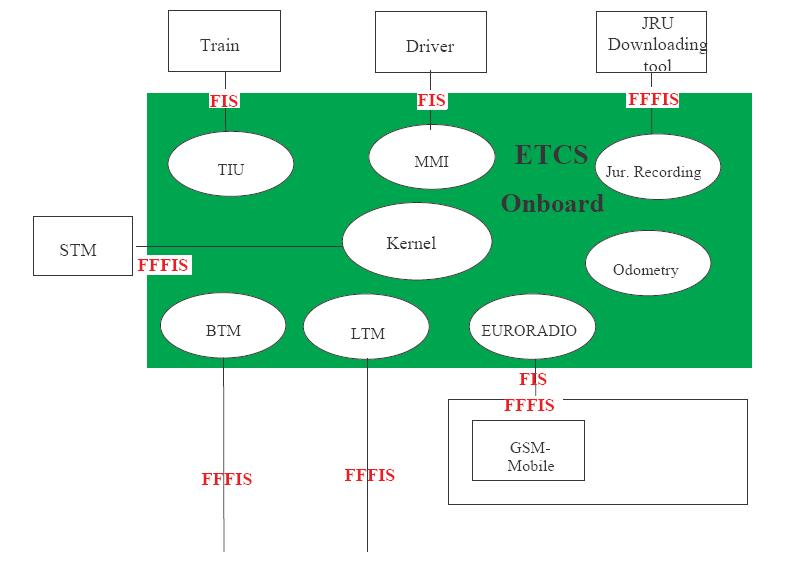
\includegraphics[width=\textwidth]{image/evc_overview}
  \caption{Overview of ETCS Onboard}
  \label{fig:Overview of ETCS Onboard}
\end{figure}
\begin{itemize}
\item MMI: this interface is in fact the DMI product, which has a non standardized interface to the EVC;
\item	TIU: this interface defined at FIS level allows the communication with the train;
\item	BTM: this interface defined at FFFIS level reads the balise telegrams;
\item	LTM: this interface defined at FFFIS level reads the loop telegrams;
\item	Euroradio (RIM): this interface defined at FFFIS level allows the communication by radio;
\item	Odometry: this module calculates the travelled distance, train speed and accelerations;
\item	JRU: this module records all events occurring in the train; the extraction of data is defined at FFFIS level;
\item	STM: this module exists in theory in two versions: national or European; it converts as far as possible national information into ETCS information, including braking the train, when appropriate. It is optional in openETCS' scope.
\end{itemize}
\section{Limitations}
The mode STM European is not supported.

\chapter{System overview}
\section{Context diagram}
\begin{figure}[!h]
  \centering
  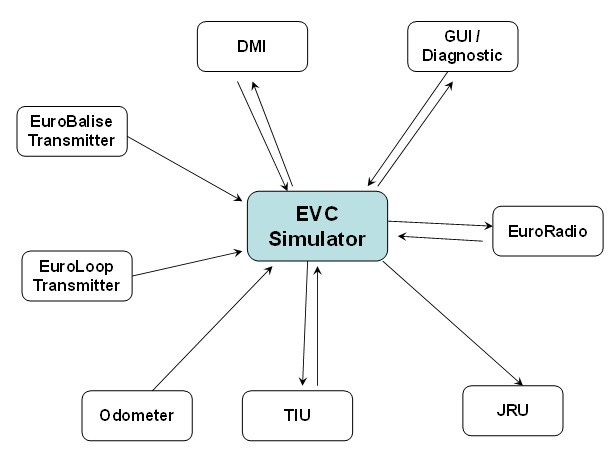
\includegraphics[width=\textwidth]{image/evc_context_diagram}
  \caption{Context diagram}
  \label{fig:Context diagram}
\end{figure}
\subsection{EVC simulator}
The EVC simulator is, fundamentally, the centre of all the control process and protection of the train movement. It performs the following main tasks:
\begin{itemize}
\item it checks the state of the system and performs all mode and level transitions;
\item it validates the data entered by the driver;
\item it calculates the train supervision curves;
\item it reads the balise, loop and radio telegrams and processes the data;
\item it validates the RBC messages and processes the data;
\item it transmits the train location and other information to the RBC;
\item it manages the movement authorities from the RBC, balises or loops;
\item it calculates the most restrictive speed limits for the current train location;
\item it supervises the train movements (including the protection against undesirable movement) and triggers warnings and interventions;
\item it records all events occurring in the system.
\end{itemize}
\subsection{EuroBalise transmitter}
The EuroBalise transmitter manages the reception of the balise messages and transmits them to the EVC simulator. The useful data are binary balise messages according to SRS Class 1 v3.3.0, Chapter 7\&8. It is a simplified BTM.
\subsection{EuroLoop transmitter}
The EuroLoop transmitter manages the reception of the loop messages and transmits them to the EVC simulator. The useful data are binary loop messages according to SRS Class 1 v3.3.0, Chapter 7\&8. It is a simplified LTM. 
\subsection{EuroRadio}
The EuroRadio manages the interface with the radio network. It manages the connection and the exchanged of data between the EVC simulator and the RBC / RIU. The exchanged data are composed of radio primitives and radio messages. The format of the exchanged messages is described in Appendix D (page \pageref{euroradio_data})
\subsection{Odometer}
The Odometer transmits to the EVC simulator the train location data (position, speed, acceleration). The odometric data are described in Appendix B (page \pageref{odometric_data})
\subsection{TIU}
The TIU manages the interface between the EVC simulator and the train equipment. It receives some commands from the EVC simulator (service brake application, emergency brake application, ...) and transmits some status (main power switch, cabin open, service brake applied, ...). The TIU data are described in  Appendix C (page \pageref{tiu_data})
\subsection{DMI}
The DMI manages the interface with the driver. It receives from the EVC simulator the information to displayed to the driver (train speed, permitted speed, track description, ...) and it transmits the driver action (train data entry, shunting request, ...).
The data are exchanged according to specification for EVC-DMI communication (see /6/).
The DMI interface is according to /6/.
\subsection{GUI/Diagnostic}
The GUI / diagnostic interface is specific to the EVC simulator. It displays the status of internal data of the EVC simulator and the operator can send some commands.
\subsection{JRU}
The JRU receives the juridical data to record. The format of the binary frame is according to /1/.

\section{Architecture diagram}
\begin{figure}[!h]
  \centering
  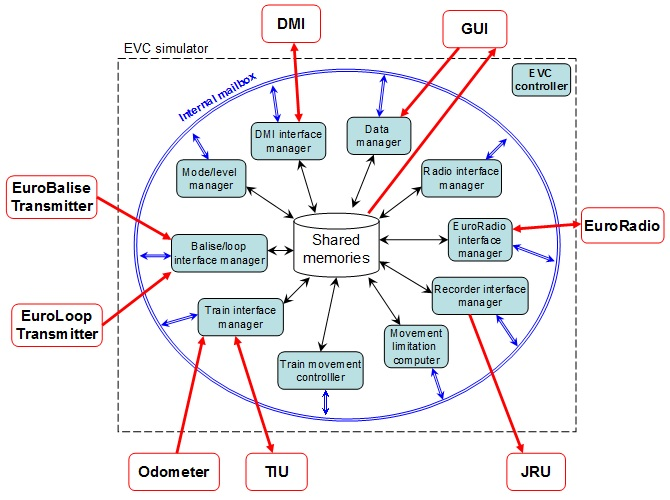
\includegraphics[width=\textwidth]{image/evc_archi_diagram}
  \caption{Architecture diagrams}
  \label{fig:Architecture diagram}
\end{figure}
The EVC simulator has been divided into 10 separate modules (a module is implemented by a periodic thread). The communication between the modules is performed via an internal mailbox and shared memories.
\begin{itemize}
\item	Train interface manager: it performs the following tasks:
	\begin{itemize}
	\item	It receives and processes the odometric data to update the internal location data.
	\item	It updates the EVC commands on the TIU.
	\item	It gets the train statuses from the TIU.
	\end{itemize}
\item	Balise/loop interface manager: it performs the following tasks:
	\begin{itemize}
	\item	It receives and decodes the balise and loop message.
	\item	It manages the balise groups.
	\item	It manages the balise linking.
	\item	It manages the track condition about big metal masses.
	\end{itemize}
\item	DMI interface manager: it performs the following tasks:
	\begin{itemize}
	\item	It manages the communication with the DMI.
	\item	It sends relevant data for display.
	\item	It manages the train data entry.
	\item	It gets the driver request.
	\end{itemize}
\item	Radio interface manager: it performs the following tasks:
	\begin{itemize}
	\item	It manages the radio session with RBC/RIU.
	\item	It receives and decodes the radio messages.
	\item	It builds and sends radio messages.
	\item	It manages the supervision of the radio link.
	\item	It manages the RBC transition.
	\end{itemize}
\item	EuroRadio interface manager: it performs the following tasks:
	\begin{itemize}
	\item It manages the communication with the EuroRadio.
	\item	It manages the safe radio connection.
	\item	It transmits the radio messages.
	\end{itemize}
\item	Recorder interface manager: it performs the following tasks:
	\begin{itemize}
	\item	It manages the recording of juridical data.
	\end{itemize}
\item	Data manager: it performs the following tasks:
	\begin{itemize}
	\item	It manages the received data from trackside: apply filter according to the ETCS mode/level and current level transition, dispatch data to the other modules.
	\item	It manages the track condition.
	\item	It manages the national data.
	\item	It manages the route suitability data.
	\item	It manages the emergency stop.
	\item	It manages the operator action on the GUI.
	\end{itemize}
\item	Movement limitation computer: it performs the following tasks:
	\begin{itemize}
	\item	It computes and provides supervision data according to ETCS mode/level.
	\item	It manages the track description: static speed profile, gradient profile, temporary speed restriction, axle load speed profile.
	\item	It manages reduction of movement authority according to conditional emergency stop, route unsuitability, mode profile.
	\end{itemize}
\item	Train movement controller: it performs the following tasks:
	\begin{itemize}
	\item	It manages the supervision of the train movement according to the ETCS mode and the available supervision data.
	\item	It manages the service brakes and emergency brakes requests.
	\item	It supervises an area according to a list of balise group (in shunting or staff responsible mode).
	\end{itemize}
\item	Mode/level manager: it performs the following tasks:
	\begin{itemize}
	\item	It manages the EVC status, ETCS mode and level.
	\item	It manages the level transition.
	\item	It manages the reversing area.
	\item	It manages the Override EOA.
	\item	It manages the mode profile.
	\end{itemize}
\end{itemize}

There is one additional module: the EVC simulator controller. It performs the following main tasks:
\begin{itemize}
\item It creates the shared memories.
\item It gets the configuration data to initialise the shared memories and to configure the EVC simulation.
\item It creates the internal mailbox of the EVC simulator.
\item It manages the start and stop of the other modules.
\end{itemize}
\chapter{Train interface manager}
\section{Overview}
The Train interface manager performs the following tasks:
\begin{itemize}
\item	It receives and processes the odometric data to update the internal location data.
\item	It updates the EVC commands on the TIU.
\item	It gets the train statuses from the TIU.
\end{itemize}
\section{Exchanged data}
This part provides a list of the main exchanged data. 
\subsection{Input data}
			\begin{longtable}{|l|l|}
				\caption{Train interface manager: Input data}\\ 
				\hline
				
					\begin{minipage}[t]{0.35\linewidth} \textbf{Source}	\end{minipage} 
				&	\begin{minipage}[t]{0.65\linewidth} \textbf{Data} \end{minipage} \\
				
				\hline
																																									
					\begin{minipage}[t]{0.35\linewidth} Odometer	\end{minipage} 
				&	\begin{minipage}[t]{0.65\linewidth}
						\begin{itemize}
							\item Estimated train position
							\item Position accuracy
							\item Estimated speed
							\item Speed accuracy
							\item Estimated acceleration
							\item Reference time
							\item Train movement direction
						\end{itemize}
					\end{minipage} \\
				
				\hline
				
					\begin{minipage}[t]{0.35\linewidth} TIU	\end{minipage} 
				&	\begin{minipage}[t]{0.65\linewidth}
						\begin{itemize}
							\item Main power switch status
							\item Train integrity status
							\item Active cabin
							\item Sleeping signal status
							\item Non leading permission
							\item Passive shunting permission
							\item Direction controller position
							\item Regenerative brake status
							\item Magnetic shoe brake status
							\item Eddy current brake status
							\item Electro Pneumatic brake status
							\item Additional brake status
							\item Train data information
							\item Type of train data entry
							\item Traction status
							\item National system isolation status
							\item Brake pressure
						\end{itemize}			
					\end{minipage} \\
				
				\hline	
				
					\begin{minipage}[t]{0.35\linewidth} Shared memories	\end{minipage} 
				&	\begin{minipage}[t]{0.65\linewidth}
						\begin{itemize}
							\item Odometry error model
							\item TIU data (outputs)
						\end{itemize}				
					\end{minipage} \\
				
				\hline	
			\end{longtable}	
\subsection{Output data}
			\begin{longtable}{|l|l|}
				\caption{Train interface manager: Output data}\\ 
				\hline
				
					\begin{minipage}[t]{0.35\linewidth} \textbf{Destination}	\end{minipage} 
				&	\begin{minipage}[t]{0.65\linewidth} \textbf{Data} \end{minipage} \\
				
				\hline
																																													
					\begin{minipage}[t]{0.35\linewidth} TIU	\end{minipage} 
				&	\begin{minipage}[t]{0.65\linewidth}
						\begin{itemize}
							\item Service Brake command
							\item Emergency Brake command
							\item Traction Cut-Off command
							\item Regenerative Brake inhibition
							\item Magnetic Shoe Brake inhibition
							\item Eddy Current Brake for SB inhibition
							\item Eddy Current Brake for EB inhibition
							\item Change of traction system
							\item Pantograph command
							\item Air Tightness command
							\item Main Power Switch command (sometimes named main circuit breaker)
							\item Isolation status
							\item Station location
							\item Allowed current consumption
						\end{itemize}			
					\end{minipage} \\
				
				\hline	
				
					\begin{minipage}[t]{0.35\linewidth} Shared memories	\end{minipage} 
				&	\begin{minipage}[t]{0.65\linewidth}
						\begin{itemize}
							\item TIU data (inputs)
							\item Train location data
						\end{itemize}				
					\end{minipage} \\
				
				\hline	
			\end{longtable}
\newpage
\section{Functions}
The following functions are performed by the Train interface manager:
\begin{figure}[!h]
  \centering
  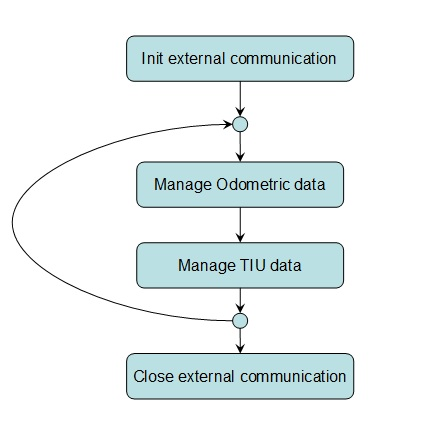
\includegraphics[width=\textwidth]{image/evc_train_interf_manager}
  \caption{Train interface manager, sequence diagram}
  \label{Train interface manager, sequence diagram}
\end{figure}

\subsection{Initialize the external communication}
It initialises the communication with the Odometer.
It initialises the communication with the TIU.
\subsection{Manage odometric data}
It gets the odometric data (position, speed, acceleration) of the train.
It calculates the internal train location data (train front location, train rear location, ...):
\begin{itemize}
	\item It converts the location data in train coordinate according to the active cabin: the distance increment direction is the train orientation defined by the active cabin.
	\item It calculates the location error according to the error model.
\end{itemize} 
It updates the train location data stored in shared memory.
\subsection{Manage TIU data}
It updates the EVC commands on TIU from data in the shared memories.
It gets the train statuses from TIU and stores them in the shared memories.
\subsection{Close the external communication}
It closes the communication with the Odometer.
It closes the communication with the TIU.
\chapter{Balise/loop interface manager}
\section{Overview}
The Balise/loop interface manager performs the following tasks:
\begin{itemize}
\item It receives and decodes the balise and loop message.
\item It manages the balise groups.
\item It manages the balise linking.
\item It manages the track condition about big metal masses.
\end{itemize}
\section{Exchanged data}
\subsection{Input data}
			\begin{longtable}{|l|l|}
				\caption{Balise/loop interface manager: Input data}\\ 
				\hline
				
					\begin{minipage}[t]{0.35\linewidth} \textbf{Source}	\end{minipage} 
				&	\begin{minipage}[t]{0.65\linewidth} \textbf{Data} \end{minipage} \\
				
				\hline
																																									
					\begin{minipage}[t]{0.35\linewidth} EuroBalise transmitter	\end{minipage} 
				&	\begin{minipage}[t]{0.65\linewidth}
						\begin{itemize}
							\item Balise message
						\end{itemize}
					\end{minipage} \\
				
				\hline
				
					\begin{minipage}[t]{0.35\linewidth} EuroLoop transmitter	\end{minipage} 
				&	\begin{minipage}[t]{0.65\linewidth}
						\begin{itemize}
							\item Loop message
						\end{itemize}
					\end{minipage} \\
				
				\hline		
						
					\begin{minipage}[t]{0.35\linewidth} Data manager	\end{minipage} 
				&	\begin{minipage}[t]{0.65\linewidth}
						\begin{itemize}
							\item Linking data
							\item Track condition about big metal masses
							\item Loop information
						\end{itemize}
					\end{minipage} \\
				
				\hline								
				
					\begin{minipage}[t]{0.35\linewidth} Shared memories	\end{minipage} 
				&	\begin{minipage}[t]{0.65\linewidth}
						\begin{itemize}
							\item Train location data
							\item Onboard status data
							\item LRBG data
							\item Train equipment						
						\end{itemize}				
					\end{minipage} \\
				
				\hline	
			\end{longtable}	
\subsection{Output data}
			\begin{longtable}{|l|l|}
				\caption{Balise/loop interface manager: Output data}\\ 
				\hline
				
					\begin{minipage}[t]{0.35\linewidth} \textbf{Destination}	\end{minipage} 
				&	\begin{minipage}[t]{0.65\linewidth} \textbf{Data} \end{minipage} \\
				
				\hline
																																									
					\begin{minipage}[t]{0.35\linewidth} Data manager	\end{minipage} 
				&	\begin{minipage}[t]{0.65\linewidth}
						\begin{itemize}
							\item Balise group message
							\item Loop message						
						\end{itemize}
					\end{minipage} \\
				
				\hline
				
					\begin{minipage}[t]{0.35\linewidth} Train movement controller	\end{minipage} 
				&	\begin{minipage}[t]{0.65\linewidth}
						\begin{itemize}
							\item Service brake application request
							\item Service brake release request
						\end{itemize}			
					\end{minipage} \\
				
				\hline
					
					\begin{minipage}[t]{0.35\linewidth} Movement limitation computer	\end{minipage} 
				&	\begin{minipage}[t]{0.65\linewidth}
						\begin{itemize}
							\item MA reduction request
						\end{itemize}			
					\end{minipage} \\
				
				\hline	
									
					\begin{minipage}[t]{0.35\linewidth} Mode/level manager	\end{minipage} 
				&	\begin{minipage}[t]{0.65\linewidth}
						\begin{itemize}
							\item Train trip request
						\end{itemize}			
					\end{minipage} \\
				
				\hline
														
					\begin{minipage}[t]{0.35\linewidth} DMI interface manager	\end{minipage} 
				&	\begin{minipage}[t]{0.65\linewidth}
						\begin{itemize}
							\item Track condition data about big metal masses
						\end{itemize}			
					\end{minipage} \\
				
				\hline																
				
					\begin{minipage}[t]{0.35\linewidth} Shared memories	\end{minipage} 
				&	\begin{minipage}[t]{0.65\linewidth}
						\begin{itemize}
							\item Current linking data
							\item LRBG data
							\item Indication of big metal masses (TIU data)						
						\end{itemize}				
					\end{minipage} \\
				
				\hline	
			\end{longtable}
\newpage				
\section{Functions}
The following functions are performed by the Balise/loop interface manager:
\begin{figure}[!h]
  \centering
  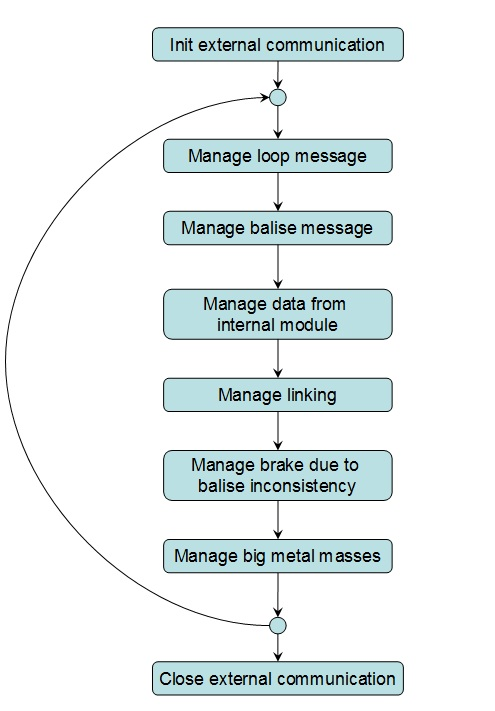
\includegraphics[width=\textwidth]{image/evc_balise_loop_interface_manager}
  \caption{Balise/loop interface manager, sequence diagram}
  \label{fig:Balise/loop interface manager, sequence diagram}
\end{figure}
\subsection{Initialize the external communication}
It initialises the communication with the EuroLoop transmitter.
It initialises the communication with the EuroBalise transmitter.
\subsection{Manage loop message}
It receives and decodes the loop messages.
It selects the data valid for the train direction according to the available information about the loop.
It transmits the decoded loop message to the data manager.

\subsection{Manage balise message}
It receives and decodes the balise messages.
It manages the balise group and checks its consistency (place of balise in group, number of balise in group).
It selects the data valid for the train direction according to the balise group orientation.
It checks the balise group linking and applies the required reaction if an inconsistency is detected.
It transmits the valid balise group message to the data manager.

\subsection{Manage data from internal module}
It receives and processes the following data from the others modules:
\begin{itemize}
\item new linking data: it is taken into account to update the current linking data used to check the balise group linking.
\item Loop information: it is stored and will be used for the management of loop message reception.
\item Track condition about big metal masses: it is taken into account to update the current list of track condition.
\end{itemize}

\subsection{Manage linking}
It checks if a balise group has not been missed according to the current linking data and performs the required reaction.

\subsection{Manage brake due to balise inconsistency}
If a service brakes application has been requested due to balise inconsistency, it manages the request for the release of the service brakes when the train reaches standstill and it request the reduction of the movement authority to the current train location.

\subsection{Manage big metal masses}
It manages the current list of track condition about big metal masses and it ignores the balise reception alarm when the balise antenna is in an area with big metal masses.

\subsection{Close the external communication}
It closes the communication with the EuroLoop transmitter.
It closes the communication with the EuroBalise transmitter.

\chapter{DMI interface manager}
\section{Overview}
The DMI interface manager performs the following tasks:
\begin{itemize}
\item It manages the communication with the DMI.
\item It sends relevant data for display.
\item It manages the train data entry.
\item It gets the driver request.
\end{itemize}
\section{Exchanged data}
\subsection{Input data}
			\begin{longtable}{|l|l|}
				\caption{DMI interface manager: Input data}\\ 
				\hline
				
					\begin{minipage}[t]{0.35\linewidth} \textbf{Source}	\end{minipage} 
				&	\begin{minipage}[t]{0.65\linewidth} \textbf{Data} \end{minipage} \\
				
				\hline
																																									
					\begin{minipage}[t]{0.35\linewidth} Data manager	\end{minipage} 
				&	\begin{minipage}[t]{0.65\linewidth}
						\begin{itemize}
							\item Track condition
							\item Text message from trackside
						\end{itemize}
					\end{minipage} \\
				
				\hline
				
					\begin{minipage}[t]{0.35\linewidth} Balise/loop interface manager\end{minipage} 
				&	\begin{minipage}[t]{0.65\linewidth}
						\begin{itemize}
							\item Track condition data about big metal masses
						\end{itemize}			
					\end{minipage} \\
				
				\hline
					
					\begin{minipage}[t]{0.35\linewidth} All modules\end{minipage} 
				&	\begin{minipage}[t]{0.65\linewidth}
						\begin{itemize}
							\item Text messages
						\end{itemize}			
					\end{minipage} \\
				
				\hline
										
					\begin{minipage}[t]{0.35\linewidth} Movement limitation computer\end{minipage} 
				&	\begin{minipage}[t]{0.65\linewidth}
						\begin{itemize}
							\item Track description (gradient profile, static speed profile, TSR)
						\end{itemize}			
					\end{minipage} \\
				
				\hline											
				
					\begin{minipage}[t]{0.35\linewidth} Shared memories	\end{minipage} 
				&	\begin{minipage}[t]{0.65\linewidth}
						\begin{itemize}
							\item On-board status data
							\item Train location data
							\item Route unsuitability indication
							\item Train data
							\item RBC data
							\item SR data
							\item TIU data
							\item Emergency stop
							\item Supervision data
							\item Radio communication status
							\item Reversing area indication
							\item Adhesion data
						\end{itemize}				
					\end{minipage} \\
				
				\hline	
			\end{longtable}	
\subsection{Output data}
			\begin{longtable}{|l|l|}
				\caption{DMI interface manager: Output data}\\ 
				\hline
				
					\begin{minipage}[t]{0.35\linewidth} \textbf{Destination}	\end{minipage} 
				&	\begin{minipage}[t]{0.65\linewidth} \textbf{Data} \end{minipage} \\
				
				\hline
																																									
					\begin{minipage}[t]{0.35\linewidth} All modules	\end{minipage} 
				&	\begin{minipage}[t]{0.65\linewidth}
						\begin{itemize}
							\item Text message acknowledgement result
						\end{itemize}
					\end{minipage} \\
				
				\hline
				
					\begin{minipage}[t]{0.35\linewidth} Train movement controller	\end{minipage} 
				&	\begin{minipage}[t]{0.65\linewidth}
						\begin{itemize}
							\item Service brake application request
							\item Service brake release request
						\end{itemize}			
					\end{minipage} \\
				
				\hline

					\begin{minipage}[t]{0.35\linewidth} Mode/level manager	\end{minipage} 
				&	\begin{minipage}[t]{0.65\linewidth}
						\begin{itemize}
							\item Driver request (start, shunting, non leading, override, ...)
							\item Data entry (driver id, level, train data, ...)
						\end{itemize}			
					\end{minipage} \\
				
				\hline	
								
					\begin{minipage}[t]{0.35\linewidth} Data manager	\end{minipage} 
				&	\begin{minipage}[t]{0.65\linewidth}
						\begin{itemize}
							\item Override route unsuitability
							\item Adhesion factor from driver
						\end{itemize}			
					\end{minipage} \\
				
				\hline	
									
					\begin{minipage}[t]{0.35\linewidth} Movement limitation computer	\end{minipage} 
				&	\begin{minipage}[t]{0.65\linewidth}
						\begin{itemize}
							\item MA reduction request 
							\item Request for new calculation of supervision data
						\end{itemize}			
					\end{minipage} \\
				
				\hline														
				
					\begin{minipage}[t]{0.35\linewidth} Shared memories	\end{minipage} 
				&	\begin{minipage}[t]{0.65\linewidth}
						\begin{itemize}
							\item RBC data
							\item Train data
							\item SR data
						\end{itemize}				
					\end{minipage} \\
				
				\hline	
			\end{longtable}
				
\newpage				
\section{Functions}
The following functions are performed by the DMI interface manager:
\begin{figure}[!h]
  \centering
  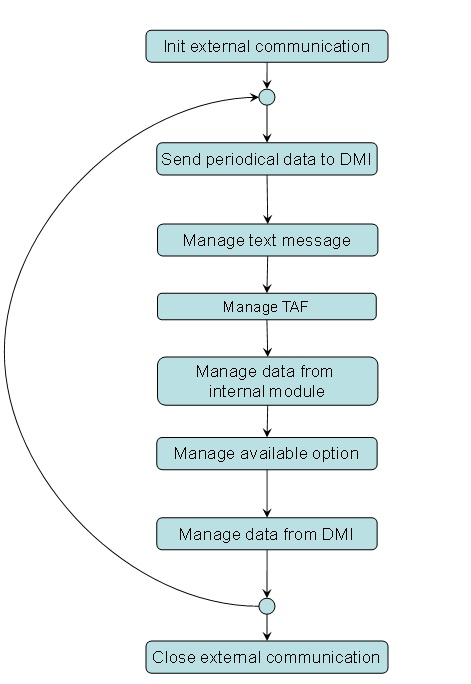
\includegraphics[width=\textwidth]{image/evc_dmi_interf_manager}
  \caption{DMI interface manager, sequence diagram}
  \label{fig:DMI interface manager, sequence diagram}
\end{figure}
\subsection{Initialize the external communication}
It initialises the communication with the DMI.
\subsection{Send periodical data to DMI}
It builds and sends a message containing some data to be updated periodically on DMI: train location, train speed, supervised speed, status of brakes, ETCS mode \& level, ...
\subsection{Manage text message}
It manages the conditions to display or remove a text message on the DMI from a list of text message.
\subsection{Manage TAF}
It manages the display, the remove of the track ahead free request. It processes the acknowledgment.

\subsection{Manage data from internal modules}
It receives and processes the following data from the others modules:
\begin{itemize}
\item New text message to display: it adds the text message in the current list of text message to manage.
\item New track description: it builds and sends a message containing the track description (static speed profile, gradient profile, track condition, ...) to the DMI.
\item Operator request via GUI: it manages the operation request performed on the GUI as it was a driver action performed on the DMI.
\end{itemize}

\subsection{Manage available option}
According to the On-board status, it builds and sends a message to the DMI containing the available option (entry of level, selection of shunting request, ...).

\subsection{Manage data from DMI}
It receives, decodes and processes the messages from the DMI:
\begin{itemize}
\item It manages the data entry (driver id, ETCS level, train data, ...) and informs the other modules.
\item It gets the driver request (Shunting request, Start of Mission request, ...) and transmits them to the suitable module.
\item It manages the text message acknowledgements.
\end{itemize}

\subsection{Close the external communication}
It closes the communication with the DMI.

\chapter{Radio interface manager}
\section{Overview}
The Radio interface manager performs the following tasks:
\begin{itemize}
\item	It manages the radio session with RBC/RIU.
\item	It receives and decodes the radio messages.
\item	It builds and sends radio messages.
\item	It manages the supervision of the radio link.
\item	It manages the RBC transition.
\end{itemize}
\section{Exchanged data}
\subsection{Input data}
			\begin{longtable}{|l|l|}
				\caption{Radio interface manager: Input data}\\ 
				\hline
				
					\begin{minipage}[t]{0.35\linewidth} \textbf{Source}	\end{minipage} 
				&	\begin{minipage}[t]{0.65\linewidth} \textbf{Data} \end{minipage} \\
				
				\hline
																																									
					\begin{minipage}[t]{0.35\linewidth} Data manager	\end{minipage} 
				&	\begin{minipage}[t]{0.65\linewidth}
						\begin{itemize}
							\item Request to send a radio message
							\item RBC transition data
							\item Radio session data
							\item RBC connection /.disconnection request
						\end{itemize}
					\end{minipage} \\
				
				\hline
				
					\begin{minipage}[t]{0.35\linewidth} Mode /level manager	\end{minipage} 
				&	\begin{minipage}[t]{0.65\linewidth}
						\begin{itemize}
							\item Request to send a radio message
							\item RBC connection /.disconnection request
						\end{itemize}			
					\end{minipage} \\
				
				\hline
					
					\begin{minipage}[t]{0.35\linewidth} EuroRadio interface manager	\end{minipage} 
				&	\begin{minipage}[t]{0.65\linewidth}
						\begin{itemize}
							\item Connection / disconnection information
							\item Radio message received
						\end{itemize}			
					\end{minipage} \\
				
				\hline	
									
					\begin{minipage}[t]{0.35\linewidth} Movement limitation computer	\end{minipage} 
				&	\begin{minipage}[t]{0.65\linewidth}
						\begin{itemize}
							\item Request to send a radio message
						\end{itemize}			
					\end{minipage} \\
				
				\hline										
				
					\begin{minipage}[t]{0.35\linewidth} Shared memories	\end{minipage} 
				&	\begin{minipage}[t]{0.65\linewidth}
						\begin{itemize}
							\item RBC data
							\item National values
							\item Train location data
							\item LRBG data
							\item Train data
						\end{itemize}				
					\end{minipage} \\
				
				\hline	
			\end{longtable}	
\subsection{Output data}
			\begin{longtable}{|l|l|}
				\caption{Radio interface manager: Output data}\\ 
				\hline
				
					\begin{minipage}[t]{0.35\linewidth} \textbf{Destination}	\end{minipage} 
				&	\begin{minipage}[t]{0.65\linewidth} \textbf{Data} \end{minipage} \\
				
				\hline
																																									
					\begin{minipage}[t]{0.35\linewidth} EuroRadio interface manager	\end{minipage} 
				&	\begin{minipage}[t]{0.65\linewidth}
						\begin{itemize}
							\item Connection /.disconnection request
							\item Request to send a radio message
						\end{itemize}
					\end{minipage} \\
				
				\hline
				
					\begin{minipage}[t]{0.35\linewidth} Mode/level manager	\end{minipage} 
				&	\begin{minipage}[t]{0.65\linewidth}
						\begin{itemize}
							\item Radio communication session open/closed
							\item Train trip request
						\end{itemize}			
					\end{minipage} \\
				
				\hline	
				
					\begin{minipage}[t]{0.35\linewidth} Train movement controller	\end{minipage} 
				&	\begin{minipage}[t]{0.65\linewidth}
						\begin{itemize}
							\item Service brake application request
							\item Service brake release request
						\end{itemize}			
					\end{minipage} \\
				
					\begin{minipage}[t]{0.35\linewidth} Movement limitation computer	\end{minipage} 
				&	\begin{minipage}[t]{0.65\linewidth}
						\begin{itemize}
							\item MA reduction request
						\end{itemize}			
					\end{minipage} \\
				
				\hline	
								
					\begin{minipage}[t]{0.35\linewidth} Data manager	\end{minipage} 
				&	\begin{minipage}[t]{0.65\linewidth}
						\begin{itemize}
							\item Received radio message
						\end{itemize}			
					\end{minipage} \\
				
				\hline	
												
				\hline					
					\begin{minipage}[t]{0.35\linewidth} Shared memories	\end{minipage} 
				&	\begin{minipage}[t]{0.65\linewidth}
						\begin{itemize}
							\item Radio communication status
							\item RBC data
						\end{itemize}				
					\end{minipage} \\
				
				\hline	
			\end{longtable}
\newpage				
\section{Functions}
The following functions are performed by the Radio interface manager:
\begin{figure}[!h]
  \centering
  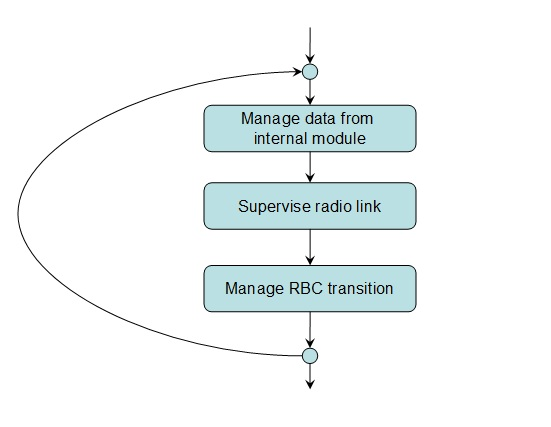
\includegraphics[width=\textwidth]{image/evc_radio_interf_manager}
  \caption{Radio interface manager, sequence diagram}
  \label{fig:Radio interface manager, sequence diagram}
\end{figure}
\subsection{Manage data from internal module}
It receives and processes the following data from the others modules:
\begin{itemize}
\item Connection / disconnection request: it manages the radio communication session establishment / termination.
\item Send message request: it builds and sends the requested message.
\item New RBC transition data: it is stored for the management of the RBC transition.
\item Connection / disconnection indication: it is taken into account for the management of the radio communication session.
\item Reception of radio message: it is decoded, the timestamp consistency is checked, it checks the used LRBG, it selects the data valid for the train direction, it manages the acknowledgement, it manages the radio communication session and it transmits the message to the Data manager.
\end{itemize}

\subsection{Supervise radio link}
According to the national values, it checks the maximum time since the last received radio message when a radio communication session is established and it applies the required reaction. It manages the radio holes.

\subsection{Manage RBC transition}
It manages the RBC transition according to the available radio equipment (one or two equipments available).

\chapter{EuroRadio interface manager}
\section{Overview}
The EuroRadio interface manager performs the following tasks:
\begin{itemize}
\item	It manages the communication with the EuroRadio.
\item	It manages the safe radio connection.
\item	It transmits the radio messages.
\end{itemize}
\section{Exchanged data}
\subsection{Input data}
			\begin{longtable}{|l|l|}
				\caption{EuroRadio interface manager: Input data}\\ 
				\hline
				
					\begin{minipage}[t]{0.35\linewidth} \textbf{Source}	\end{minipage} 
				&	\begin{minipage}[t]{0.65\linewidth} \textbf{Data} \end{minipage} \\
				
				\hline
																																									
					\begin{minipage}[t]{0.35\linewidth} EuroRadio	\end{minipage} 
				&	\begin{minipage}[t]{0.65\linewidth}
						\begin{itemize}
							\item Connection/disconnection indication
							\item Reception of radio message
						\end{itemize}
					\end{minipage} \\
				
				\hline
				
					\begin{minipage}[t]{0.35\linewidth} Radio interface manager	\end{minipage} 
				&	\begin{minipage}[t]{0.65\linewidth}
						\begin{itemize}
							\item Connection/disconnection request
							\item Request to send a radio message
						\end{itemize}			
					\end{minipage} \\
				
				\hline	
			\end{longtable}	
\subsection{Output data}
			\begin{longtable}{|l|l|}
				\caption{EuroRadio interface manager: Output data}\\ 
				\hline
				
					\begin{minipage}[t]{0.35\linewidth} \textbf{Destination}	\end{minipage} 
				&	\begin{minipage}[t]{0.65\linewidth} \textbf{Data} \end{minipage} \\
				
				\hline
																																									
					\begin{minipage}[t]{0.35\linewidth} Radio interface manager	\end{minipage} 
				&	\begin{minipage}[t]{0.65\linewidth}
						\begin{itemize}
							\item Connection / disconnection information
							\item Radio message received
						\end{itemize}
					\end{minipage} \\
				
				\hline
				
					\begin{minipage}[t]{0.35\linewidth} EuroRadio	\end{minipage} 
				&	\begin{minipage}[t]{0.65\linewidth}
						\begin{itemize}
							\item Connection / disconnection request
							\item Transmission of radio message request
						\end{itemize}			
					\end{minipage} \\
				
				\hline	
				
					\begin{minipage}[t]{0.35\linewidth} Shared memories	\end{minipage} 
				&	\begin{minipage}[t]{0.65\linewidth}
						\begin{itemize}
							\item Radio connection status
						\end{itemize}				
					\end{minipage} \\
				
				\hline	
			\end{longtable}
\newpage				
\section{Functions}
The following functions are performed by the EuroRadio interface manager:
\begin{figure}[!h]
  \centering
  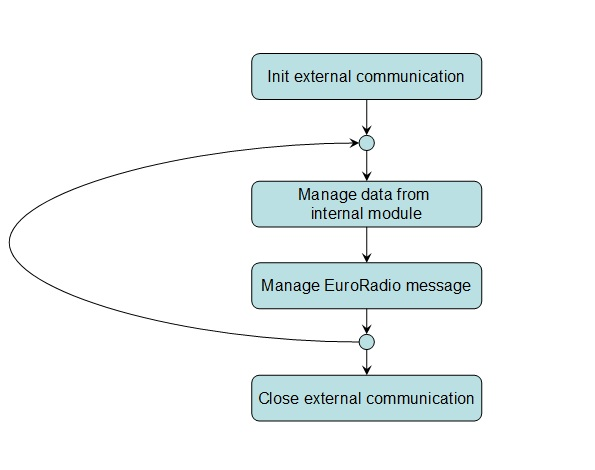
\includegraphics[width=\textwidth]{image/evc_euroradio_interf_manager}
  \caption{EuroRadio interface manager, sequence diagram}
  \label{fig:EuroRadio interface manager, sequence diagram}
\end{figure}
\subsection{Initialize the external communication}
It initialises the communication with the EuroRadio.
\subsection{Manage data from internal module}
It receives and processes the following data from the others modules:
\begin{itemize}
\item Connection/disconnection request: it builds and sends the message for the connection/disconnection request to the EuroRadio.
\item Data send request: it builds and sends the message for the data send request to the EuroRadio.
\end{itemize}
\subsection{Manage EuroRadio message}
It receives and decodes the messages from the EuroRadio, it manages the radio connection and it informs the Radio interface manager of the connection/disconnection and reception of radio message.
\subsection{Close the external communication}
It closes the communication with the EuroRadio.

\chapter{Recorder interface manager}
\section{Overview}
The Recorder interface manager performs the following tasks:
\begin{itemize}
\item	It manages the recording of juridical data.
\end{itemize}

\section{Exchanged data}
\subsection{Input data}
			\begin{longtable}{|l|l|}
				\caption{Recorder interface manager: Input data}\\ 
				\hline
				
					\begin{minipage}[t]{0.35\linewidth} \textbf{Source}	\end{minipage} 
				&	\begin{minipage}[t]{0.65\linewidth} \textbf{Data} \end{minipage} \\
				
				\hline
																																									
					\begin{minipage}[t]{0.35\linewidth} All modules	\end{minipage} 
				&	\begin{minipage}[t]{0.65\linewidth}
						\begin{itemize}
							\item Juridical event to record
						\end{itemize}
					\end{minipage} \\
				
				\hline
				
					\begin{minipage}[t]{0.35\linewidth} Shared memories	\end{minipage} 
				&	\begin{minipage}[t]{0.65\linewidth}
						\begin{itemize}
							\item ETCS mode \& level (on-board status)
							\item Train location data
						\end{itemize}				
					\end{minipage} \\
				
				\hline	
			\end{longtable}	
\subsection{Output data}
			\begin{longtable}{|l|l|}
				\caption{Recorder interface manager: Output data}\\ 
				\hline
				
					\begin{minipage}[t]{0.35\linewidth} \textbf{Destination}	\end{minipage} 
				&	\begin{minipage}[t]{0.65\linewidth} \textbf{Data} \end{minipage} \\
				
				\hline
																																									
					\begin{minipage}[t]{0.35\linewidth} JRU	\end{minipage} 
				&	\begin{minipage}[t]{0.65\linewidth}
						\begin{itemize}
							\item Juridical data to record
						\end{itemize}
					\end{minipage} \\
				
				\hline
			\end{longtable}
\newpage				
\section{Functions}
The following functions are performed by the Recorder interface manager:
\begin{figure}[!h]
  \centering
  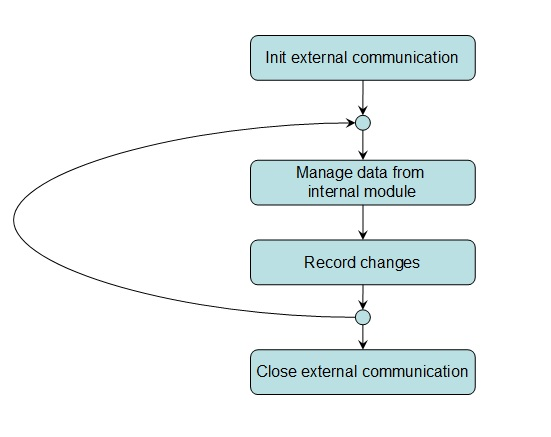
\includegraphics[width=\textwidth]{image/evc_recorder_interf_manager}
  \caption{Recorder interface manager, sequence diagram}
  \label{fig:Recorder interface manager, sequence diagram}
\end{figure}
\subsection{Initialize the external communication}
It initialises the communication with the JRU.
\subsection{Manage data from internal module}
It receives the juridical event to record: it builds and sends the corresponding message to the JRU.
\subsection{Record changes}
It builds and sends message to the JRU for the record of periodical data (train location , speed, ...) or when a juridical data changes (ETCS mode, level, ...)
\subsection{Close the external communication}
It closes the communication with the JRU.
\chapter{Data manager}
\section{Overview}
The Data manager performs the following tasks:
\begin{itemize}
\item	It manages the received data from trackside: apply filter according to the ETCS mode/level and current level transition, dispatch data to the other modules.
\item	It manages the track condition.
\item	It manages the national data.
\item	It manages the route suitability data.
\item	It manages the emergency stop.
\item	It manages the user interface and the information to display.
\end{itemize}

\section{Exchanged data}
\subsection{Input data}
			\begin{longtable}{|l|l|}
				\caption{Data manager: Input data}\\ 
				\hline
				
					\begin{minipage}[t]{0.35\linewidth} \textbf{Source}	\end{minipage} 
				&	\begin{minipage}[t]{0.65\linewidth} \textbf{Data} \end{minipage} \\
				
				\hline
																																									
					\begin{minipage}[t]{0.35\linewidth} Balise/loop interface manager	\end{minipage} 
				&	\begin{minipage}[t]{0.65\linewidth}
						\begin{itemize}
							\item Balise group message
							\item Loop message						
						\end{itemize}
					\end{minipage} \\
				
				\hline
				
					\begin{minipage}[t]{0.35\linewidth} DMI interface manager	\end{minipage} 
				&	\begin{minipage}[t]{0.65\linewidth}
						\begin{itemize}
							\item Override route unsuitability
							\item Adhesion factor from driver
						\end{itemize}			
					\end{minipage} \\
				
				\hline
					
					\begin{minipage}[t]{0.35\linewidth} Mode/level manager	\end{minipage} 
				&	\begin{minipage}[t]{0.65\linewidth}
						\begin{itemize}
							\item MA request
						\end{itemize}			
					\end{minipage} \\
				
				\hline	

					\begin{minipage}[t]{0.35\linewidth} Radio interface manager	\end{minipage} 
				&	\begin{minipage}[t]{0.65\linewidth}
						\begin{itemize}
							\item Received radio message
						\end{itemize}			
					\end{minipage} \\
				
				\hline	

					\begin{minipage}[t]{0.35\linewidth} Movement limitation computer	\end{minipage} 
				&	\begin{minipage}[t]{0.65\linewidth}
						\begin{itemize}
							\item MA request
						\end{itemize}			
					\end{minipage} \\
				
				\hline													
				
					\begin{minipage}[t]{0.35\linewidth} Shared memories	\end{minipage} 
				&	\begin{minipage}[t]{0.65\linewidth}
						\begin{itemize}
							\item On-board status data
							\item Level transition data
							\item Train location data
							\item Train data
							\item LRBG data
							\item Current linking data
							\item RBC data
						\end{itemize}				
					\end{minipage} \\
				
				\hline	
			\end{longtable}	
\subsection{Output data}
			\begin{longtable}{|l|l|}
				\caption{Data manager: Output data}\\ 
				\hline
				
					\begin{minipage}[t]{0.35\linewidth} \textbf{Destination}	\end{minipage} 
				&	\begin{minipage}[t]{0.65\linewidth} \textbf{Data} \end{minipage} \\
				
				\hline
																																									
					\begin{minipage}[t]{0.35\linewidth} Movement limitation computer	\end{minipage} 
				&	\begin{minipage}[t]{0.65\linewidth}
						\begin{itemize}
							\item Route unsuitability data
							\item Indication of new national data
							\item Repositioning information
							\item Track description (gradient, speed profile, ...)
							\item Mode profile
							\item Reversing supervision data
							\item Temporary speed restriction
							\item MA revocation request
							\item MA
							\item Emergency stop						
						\end{itemize}
					\end{minipage} \\
				
				\hline
				
					\begin{minipage}[t]{0.35\linewidth} DMI interface manager	\end{minipage} 
				&	\begin{minipage}[t]{0.65\linewidth}
						\begin{itemize}
							\item Track condition
							\item Text message from trackside
						\end{itemize}			
					\end{minipage} \\
				
				\hline
					
					\begin{minipage}[t]{0.35\linewidth} Radio interface manager	\end{minipage} 
				&	\begin{minipage}[t]{0.65\linewidth}
						\begin{itemize}
							\item Request to send radio message
							\item RBC transition data
							\item Radio session data
							\item Connection / disconnection request
						\end{itemize}			
					\end{minipage} \\
				
				\hline
									
					\begin{minipage}[t]{0.35\linewidth} Mode/level manager	\end{minipage} 
				&	\begin{minipage}[t]{0.65\linewidth}
						\begin{itemize}
							\item Level transition data
							\item RBC answer (ack of train data, Shunting accepted/rejected, ...)
							\item Mode profile
							\item Train trip request
							\item Reversing area data
						\end{itemize}			
					\end{minipage} \\
				
				\hline
													
					\begin{minipage}[t]{0.35\linewidth} Train movement controller	\end{minipage} 
				&	\begin{minipage}[t]{0.65\linewidth}
						\begin{itemize}
							\item Shunting area data
							\item Staff responsible area data
							\item Service brakes application request
							\item Service brakes release request
							\item Emergency brakes application request
							\item Emergency brakes release request
							\item New balise group indication
						\end{itemize}			
					\end{minipage} \\
				
				\hline
																	
					\begin{minipage}[t]{0.35\linewidth} Balise/loop interface manager	\end{minipage} 
				&	\begin{minipage}[t]{0.65\linewidth}
						\begin{itemize}
							\item Linking data
							\item Loop information
							\item Track condition about big metal masses
						\end{itemize}			
					\end{minipage} \\
				
				\hline
																																									
					\begin{minipage}[t]{0.35\linewidth} Shared memories	\end{minipage} 
				&	\begin{minipage}[t]{0.65\linewidth}
						\begin{itemize}
							\item Track condition data
							\item Main circuit breaker open request (TIU data)
							\item Pantograph low request (TIU data)
							\item Inhibition of passenger emergency brakes request (TIU data)
							\item Airtight request (TIU data)
							\item Switch off regenerative brakes request (TIU data)
							\item Switch off eddy current brakes request (TIU data)
							\item Switch off magnetic shoe brakes request (TIU data)
							\item National data
							\item Adhesion data
							\item Radio communication session status
						\end{itemize}				
					\end{minipage} \\
				
				\hline	
			\end{longtable}
\newpage				
\section{Functions}
The following functions are performed by the Data manager:
\begin{figure}[!h]
  \centering
  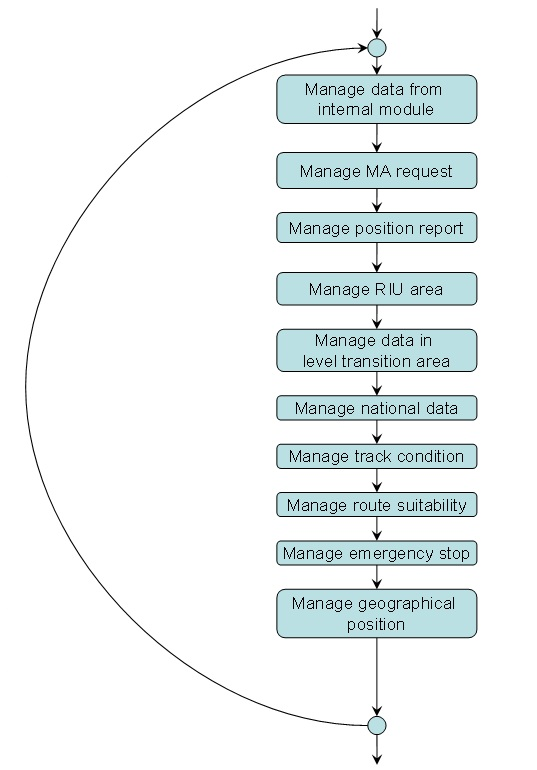
\includegraphics[width=\textwidth]{image/evc_data_manager}
  \caption{Data manager, sequence diagram}
  \label{fig:Data manager, sequence diagram}
\end{figure}
\subsection{Manage data from internal modules}
It receives the balise group message, loop message and radio message. It filters the data according to the current ETCS mode and level. It dispatches the valid data to the other modules.
It receives and manages the request for override of route unsuitability.

\subsection{Manage MA request}
It manages the sending request of the "`MA request"' radio message to the RBC according to the MA request parameters.

\subsection{Manage position report}
It manages the sending request of the "`position report"' radio message to the RBC according to the position report parameters.

\subsection{Manage RIU area}
It manages the entry / exit in the radio infill area. It manages the sending request of "`infill MA request"' radio message.

\subsection{Manage data in level transition area}
It manages the data stored in buffer during the level transition when the train enters in the new level.

\subsection{Manage national data}
It manages the national data, it checks when the new national data becomes valid, it checks the validity of the current national data, it sets the default national data.

\subsection{Manage track conditions}
It manages the list of the track condition and checks when the train enters /exits in a track condition area. It sets the TIU output required by the active track condition (switch off eddy current brakes, ...).

\subsection{Manage route suitability}
It manages the list of route suitability, it detects if there is an unsuitability according to the train data, it requests the reduction of the MA to the next unsuitability, it manages the override of the unsuitability.

\subsection{Manage emergency stop}
It manages the list of the active emergency stop.
It manages the train trip request due to unconditional emergency stop, it manages the MA reduction due to conditional emergency stop.
It manages the acknowledgement of the emergency stop and the revocation of the emergency stop.

\subsection{Manage geographical position}
It manages the received geographical data in order to calculate the corresponding KP to the train location.

\chapter{Movement limitation computer}
\section{Overview}
The Movement limitation computer performs the following tasks:
\begin{itemize}
\item	It computes and provides supervision data according to ETCS mode/level.
\item	It manages the track description: static speed profile, gradient profile, temporary speed restriction, axle load speed profile.
\item	It manages reduction of movement authority according to conditional emergency stop, route unsuitability, mode profile. 
\end{itemize}
\section{Exchanged data}
\subsection{Input data}
			\begin{longtable}{|l|l|}
				\caption{Movement limitation computer: Input data}\\ 
				\hline
				
					\begin{minipage}[t]{0.35\linewidth} \textbf{Source}	\end{minipage} 
				&	\begin{minipage}[t]{0.65\linewidth} \textbf{Data} \end{minipage} \\
				
				\hline
																																									
					\begin{minipage}[t]{0.35\linewidth} Balise/loop interface manager	\end{minipage} 
				&	\begin{minipage}[t]{0.65\linewidth}
						\begin{itemize}
							\item MA reduction request
						\end{itemize}
					\end{minipage} \\
				
				\hline
				
					\begin{minipage}[t]{0.35\linewidth} DMI interface manager	\end{minipage} 
				&	\begin{minipage}[t]{0.65\linewidth}
						\begin{itemize}
							\item MA reduction request 
							\item Request for new calculation of supervision data
						\end{itemize}			
					\end{minipage} \\
				
				\hline
				
					\begin{minipage}[t]{0.35\linewidth} Radio interface manager	\end{minipage} 
				&	\begin{minipage}[t]{0.65\linewidth}
						\begin{itemize}
							\item MA reduction request
						\end{itemize}			
					\end{minipage} \\
				
				\hline	
									
					\begin{minipage}[t]{0.35\linewidth} Data manager	\end{minipage} 
				&	\begin{minipage}[t]{0.65\linewidth}
						\begin{itemize}
							\item Route unsuitability data
							\item Indication of new national data
							\item Repositioning information
							\item Track description (gradient, speed profile, ...)
							\item Mode profile
							\item Reversing supervision data
							\item Temporary speed restriction
							\item MA revocation request
							\item MA
							\item Emergency stop
						\end{itemize}			
					\end{minipage} \\
				
				\hline	
													
					\begin{minipage}[t]{0.35\linewidth} Mode/level manager	\end{minipage} 
				&	\begin{minipage}[t]{0.65\linewidth}
						\begin{itemize}
							\item Request to calculate supervision data
						\end{itemize}			
					\end{minipage} \\
				
				\hline														
				
					\begin{minipage}[t]{0.35\linewidth} Shared memories	\end{minipage} 
				&	\begin{minipage}[t]{0.65\linewidth}
						\begin{itemize}
							\item Train data
							\item National data
							\item On-board status data
							\item Train location data
							\item Adhesion data
							\item SR data						
						\end{itemize}				
					\end{minipage} \\
				
				\hline	
			\end{longtable}	
\subsection{Output data}
			\begin{longtable}{|l|l|}
				\caption{Movement limitation computer: Output data}\\ 
				\hline
				
					\begin{minipage}[t]{0.35\linewidth} \textbf{Destination}	\end{minipage} 
				&	\begin{minipage}[t]{0.65\linewidth} \textbf{Data} \end{minipage} \\
				
				\hline
																																									
					\begin{minipage}[t]{0.35\linewidth} DMI interface manager	\end{minipage} 
				&	\begin{minipage}[t]{0.65\linewidth}
						\begin{itemize}
							\item Track description (gradient profile, static speed profile, TSR)
						\end{itemize}
					\end{minipage} \\
				
				\hline
				
					\begin{minipage}[t]{0.35\linewidth} Radio interface manager	\end{minipage} 
				&	\begin{minipage}[t]{0.65\linewidth}
						\begin{itemize}
							\item Request to send a radio message
						\end{itemize}			
					\end{minipage} \\
				
				\hline
					
					\begin{minipage}[t]{0.35\linewidth} Data manager	\end{minipage} 
				&	\begin{minipage}[t]{0.65\linewidth}
						\begin{itemize}
							\item MA request
						\end{itemize}			
					\end{minipage} \\
				
				\hline	

					\begin{minipage}[t]{0.35\linewidth} Mode/Level manager 	\end{minipage} 
				&	\begin{minipage}[t]{0.65\linewidth}
						\begin{itemize}
							\item Indication of MA valid
						\end{itemize}			
					\end{minipage} \\
				
				\hline
				
					\begin{minipage}[t]{0.35\linewidth} Shared memories	\end{minipage} 
				&	\begin{minipage}[t]{0.65\linewidth}
						\begin{itemize}
							\item Supervision data
						\end{itemize}				
					\end{minipage} \\
				
				\hline	
			\end{longtable}
\newpage				
\section{Functions}
The following functions are performed by the Movement limitation computer:
\begin{figure}[!h]
  \centering
  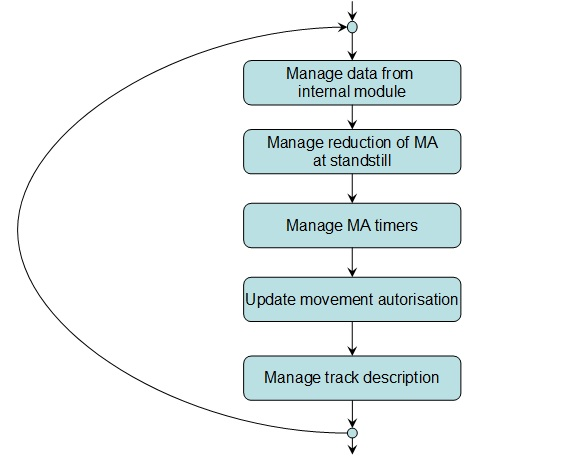
\includegraphics[width=\textwidth]{image/evc_mvmt_limitation_computer}
  \caption{Movement limitation computer, sequence diagram}
  \label{fig:Movement limitation computer, sequence diagram}
\end{figure}
\subsection{Manage data from internal module}
It manages the reception of data from other modules:
\begin{itemize}
\item Track description data (static speed profile, gradient profile, temporary speed restriction, axle load speed profile, ...). It is stored and used for the calculation of the supervision data.
\item MA data, SR data, reversing supervision data: it is stored and used for the calculation of the supervision data.
\item Reduction due to route unsuitability: it stored and used to reduce the current MA to the location of the route unsuitability.
\item Mode profile: it is stored and used for the calculation of the supervision data.
\item Request to reduce MA to standstill location: it is stored.
\item Cooperative MA revocation request: it is processed in order to check if the train can be stopped before the new EOA.
\item Emergency stop data: it manages the stop location due to a conditional emergency stop. It is taken into account for the calculation of the supervision data.
\end{itemize}

\subsection{Manage reduction of MA at standstill}
When a request to reduce the current MA to the standstill location has been received, it checks if the train has reached standstill and it requests the calculation of supervision curves for the new reduced MA.

\subsection{Manage MA timers}
It manages the timers associated to the current MA. 
It manages the start and the stop of the timers. If there is a timer expiration, it requests the calculation of supervision curves for the modified MA data.

\subsection{Update movement authorization}
It requests the calculation of the suitable supervision data according to the current ETCS mode. The new calculation can be due to a mode change, the use of new national data or the modification of the input data (staff responsible speed/distance, reversing supervision data, MA, track description, ...).

\subsection{Manage track description}
It manages the deletion of a part or the whole track description data according to the change of the stop location and the ETCS mode.

\chapter{Train movement controller}
\section{Overview}
The Train movement controller performs the following tasks:
\begin{itemize}
\item	It manages the supervision of the train movement according to the ETCS mode and the available supervision data.
\item	It manages the service brake and emergency brake application requests.
\item	It supervises an area according to a list of balise group (in shunting or staff responsible mode).
\end{itemize}
\section{Exchanged data}
\subsection{Input data}
			\begin{longtable}{|l|l|}
				\caption{Train movement controller: Input data}\\ 
				\hline
				
					\begin{minipage}[t]{0.35\linewidth} \textbf{Source}	\end{minipage} 
				&	\begin{minipage}[t]{0.65\linewidth} \textbf{Data} \end{minipage} \\
				
				\hline
																																									
					\begin{minipage}[t]{0.35\linewidth} Data manager	\end{minipage} 
				&	\begin{minipage}[t]{0.65\linewidth}
						\begin{itemize}
							\item Shunting area data
							\item Staff responsible area data
							\item Service brakes application request
							\item Service brakes release request
							\item Emergency brakes application request
							\item Emergency brakes release request
							\item New balise group indication
						\end{itemize}
					\end{minipage} \\
				
				\hline
				
					\begin{minipage}[t]{0.35\linewidth} Radio interface manager	\end{minipage} 
				&	\begin{minipage}[t]{0.65\linewidth}
						\begin{itemize}
							\item Service brake application request
							\item Service brake release request
						\end{itemize}			
					\end{minipage} \\
				
				\hline	
				
					\begin{minipage}[t]{0.35\linewidth} DMI interface manager	\end{minipage} 
				&	\begin{minipage}[t]{0.65\linewidth}
						\begin{itemize}
							\item Service brake application request
							\item Service brake release request
						\end{itemize}			
					\end{minipage} \\
				
				\hline
					
					\begin{minipage}[t]{0.35\linewidth} Mode/Level manager 	\end{minipage} 
				&	\begin{minipage}[t]{0.65\linewidth}
						\begin{itemize}
							\item Service brake application request
							\item Service brake release request
						\end{itemize}			
					\end{minipage} \\
				
				\hline	
				
					\begin{minipage}[t]{0.35\linewidth} Balise/loop interface manager 	\end{minipage} 
				&	\begin{minipage}[t]{0.65\linewidth}
						\begin{itemize}
							\item Service brake application request
							\item Service brake release request
						\end{itemize}			
					\end{minipage} \\
				
				\hline
				
					\begin{minipage}[t]{0.35\linewidth} Shared memories	\end{minipage} 
				&	\begin{minipage}[t]{0.65\linewidth}
						\begin{itemize}
							\item Train location data
							\item On-board status data
							\item Supervision data
							\item Direction controller position (TIU data)
							\item Emergency brakes status (TIU data)
							\item Service brakes status (TIU data)
						\end{itemize}				
					\end{minipage} \\
				
				\hline	
			\end{longtable}	
\subsection{Output data}
			\begin{longtable}{|l|l|}
				\caption{Train movement controller: Output data}\\ 
				\hline
				
					\begin{minipage}[t]{0.35\linewidth} \textbf{Destination}	\end{minipage} 
				&	\begin{minipage}[t]{0.65\linewidth} \textbf{Data} \end{minipage} \\
				
				\hline
																																									
					\begin{minipage}[t]{0.35\linewidth} Mode/level manager	\end{minipage} 
				&	\begin{minipage}[t]{0.65\linewidth}
						\begin{itemize}
							\item Train trip request
						\end{itemize}
					\end{minipage} \\
				
				\hline
				
					\begin{minipage}[t]{0.35\linewidth} Radio interface manager	\end{minipage} 
				&	\begin{minipage}[t]{0.65\linewidth}
						\begin{itemize}
							\item Request to send a radio message
						\end{itemize}			
					\end{minipage} \\
				
				\hline	
				
					\begin{minipage}[t]{0.35\linewidth} Shared memories	\end{minipage} 
				&	\begin{minipage}[t]{0.65\linewidth}
						\begin{itemize}
							\item Current supervision speeds
							\item Target data
							\item Traction cut off request (TIU data)
							\item Service brakes application request (TIU data)
							\item Emergency brakes application request (TIU data)
						\end{itemize}				
					\end{minipage} \\
				
				\hline	
			\end{longtable}
\newpage				
\section{Functions}
The following functions are performed by the Train movement controller:
\begin{figure}[!h]
  \centering
  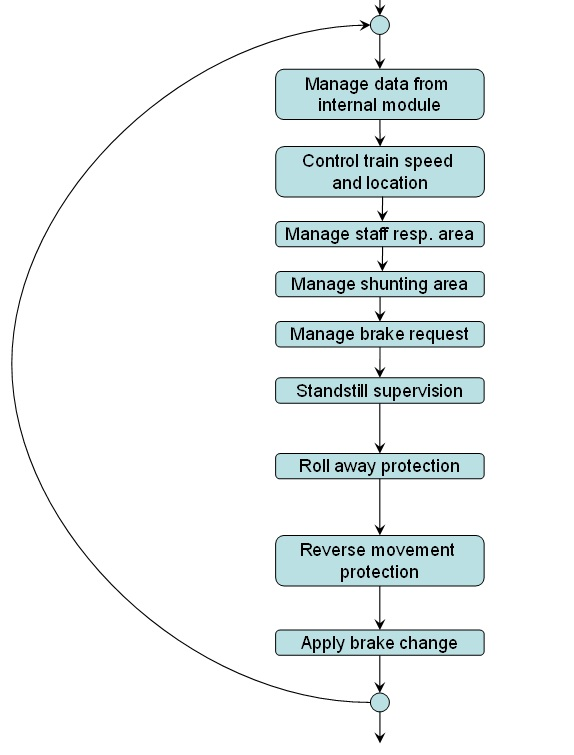
\includegraphics[width=\textwidth]{image/evc_train_mvmt_controller}
  \caption{Train movement controller, sequence diagram}
  \label{fig:Train movement controller, sequence diagram}
\end{figure}
\subsection{Manage data from internal module}
It manages the reception of data from other modules:
\begin{itemize}
\item Service brakes/emergency brakes application/release request from another module: it stores the request.
\item Shunting area data: it stores the list of balise group composing the area.
\item Staff responsible area data: it stores the list of balise group composing the area.
\item Indication of a new balise group: if the current ETCS mode is shunting or staff responsible, it checks if the passed balise group belong to the authorised area.
\item Driver acknowledgement: it processed the acknowledgement for release of brakes application (roll away protection, standstill supervision, reverse movement protection).
\end{itemize}

\subsection{Control train speed and location}
According to the supervision data, it supervises the train speed and location. 
It requests the brakes application / release for the control of the train speed. 
It can send a train trip request to the mode manager when the train is not at an authorised location.
It updates the supervision speeds and the target data in the shared memory.

\subsection{Manage brake request}
It manages the requests to apply / release the brakes received from the other modules.

\subsection{Standstill supervision}
According to the ETCS mode, it manages the standstill supervision.
It applies the brakes when a movement is detected. It releases the brakes when the intervention is acknowledged by the driver and the train is at standstill.

\subsection{Roll away protection}
According to the ETCS mode, it manages the roll away protection. 
It applies the brakes when a roll away movement is detected according to the direction controller position. It releases the brakes when the intervention is acknowledged by the driver and the train is at standstill.

\subsection{Reverse movement protection}
According to the ETCS mode, it manages the reverse movement protection. 
It applies the brakes when a reverse movement is detected. It releases the brakes when the intervention is acknowledged by the driver and the train is at standstill.

\subsection{Apply brake change}
According to the brake requests, it updates the brakes commands of the TIU outputs in the shared memory. 
It takes into account the previous brakes commands when some brakes application should be released only at standstill.
It requests the emergency brakes application when the service brakes application fails.

\chapter{Mode/level manager}
\section{Overview}
The Mode/level manager performs the following tasks:
\begin{itemize}
\item	It manages the EVC status, ETCS mode and level.
\item	It manages the level transition.
\item	It manages the reversing area.
\item	It manages the Override EOA.
\item	It manages the mode profile.
\end{itemize}
\section{Exchanged data}
\subsection{Input data}
			\begin{longtable}{|l|l|}
				\caption{Mode/level manager: Input data}\\ 
				\hline
				
					\begin{minipage}[t]{0.35\linewidth} \textbf{Source}	\end{minipage} 
				&	\begin{minipage}[t]{0.65\linewidth} \textbf{Data} \end{minipage} \\
				
				\hline
																																									
					\begin{minipage}[t]{0.35\linewidth} Movement limitation computer	\end{minipage} 
				&	\begin{minipage}[t]{0.65\linewidth}
						\begin{itemize}
							\item Indication of MA valid 
						\end{itemize}
					\end{minipage} \\
				
				\hline
				
					\begin{minipage}[t]{0.35\linewidth} Data manager	\end{minipage} 
				&	\begin{minipage}[t]{0.65\linewidth}
						\begin{itemize}
							\item Level transition data
							\item RBC answer (ack of train data, shunting accepted/rejected, ...)
							\item Mode profile
							\item Train trip request
							\item Reversing area data
						\end{itemize}			
					\end{minipage} \\
				
				\hline
					
					\begin{minipage}[t]{0.35\linewidth} DMI interface manager	\end{minipage} 
				&	\begin{minipage}[t]{0.65\linewidth}
						\begin{itemize}
							\item Driver request (shunting, start of mission, entry of level, ...)
							\item Data entry (driver id, level, train data, ...)
						\end{itemize}			
					\end{minipage} \\
				
				\hline	
									
	
					\begin{minipage}[t]{0.35\linewidth} Balise/loop interface manager	\end{minipage} 
				&	\begin{minipage}[t]{0.65\linewidth}
						\begin{itemize}
							\item Train trip request
						\end{itemize}			
					\end{minipage} \\
				
				\hline
													
					\begin{minipage}[t]{0.35\linewidth} Radio interface manager	\end{minipage} 
				&	\begin{minipage}[t]{0.65\linewidth}
						\begin{itemize}
							\item Radio communication session open/closed
							\item Train trip request
						\end{itemize}			
					\end{minipage} \\
				
				\hline
																	
																	
					\begin{minipage}[t]{0.35\linewidth} Train movement controller	\end{minipage} 
				&	\begin{minipage}[t]{0.65\linewidth}
						\begin{itemize}
							\item Train trip request
						\end{itemize}			
					\end{minipage} \\
				
				\hline	
				
					\begin{minipage}[t]{0.35\linewidth} Shared memories	\end{minipage} 
				&	\begin{minipage}[t]{0.65\linewidth}
						\begin{itemize}
							\item Main power switch status (TIU data)
							\item Active cabin (TIU data)
							\item Isolation status (TIU data)
							\item Sleeping signal status (TIU data)
							\item Train location data
							\item National data
							\item Train equipment data
							\item Radio communication status						
						\end{itemize}				
					\end{minipage} \\
				
				\hline	
			\end{longtable}	
\subsection{Output data}
			\begin{longtable}{|l|l|}
				\caption{Mode/level manager: Output data}\\ 
				\hline
				
					\begin{minipage}[t]{0.35\linewidth} \textbf{Destination}	\end{minipage} 
				&	\begin{minipage}[t]{0.65\linewidth} \textbf{Data} \end{minipage} \\
				
				\hline
																																									
					\begin{minipage}[t]{0.35\linewidth} Radio message	\end{minipage} 
				&	\begin{minipage}[t]{0.65\linewidth}
						\begin{itemize}
							\item Request to send a radio message
							\item RBC connection/disconnection request
						\end{itemize}
					\end{minipage} \\
				
				\hline
				
					\begin{minipage}[t]{0.35\linewidth} Data manager	\end{minipage} 
				&	\begin{minipage}[t]{0.65\linewidth}
						\begin{itemize}
							\item MA request
						\end{itemize}			
					\end{minipage} \\
				
				\hline
					
					\begin{minipage}[t]{0.35\linewidth} Movement limitation computer	\end{minipage} 
				&	\begin{minipage}[t]{0.65\linewidth}
						\begin{itemize}
							\item Request to calculate supervision data
						\end{itemize}			
					\end{minipage} \\
				
				\hline
				
					\begin{minipage}[t]{0.35\linewidth} Train movement controller	\end{minipage} 
				&	\begin{minipage}[t]{0.65\linewidth}
						\begin{itemize}
							\item Service brake application request
							\item Service brake release request
						\end{itemize}			
					\end{minipage} \\
				
				\hline
				
					\begin{minipage}[t]{0.35\linewidth} Shared memories	\end{minipage} 
				&	\begin{minipage}[t]{0.65\linewidth}
						\begin{itemize}
							\item On-board status data
							\item Train data status
							\item Reversing area indication
							\item Dead man isolation request (TIU data)
						\end{itemize}				
					\end{minipage} \\
				
				\hline	
			\end{longtable}
\newpage				
\section{Functions}
The following functions are performed by the Mode/level manager:
\begin{figure}[!h]
  \centering
  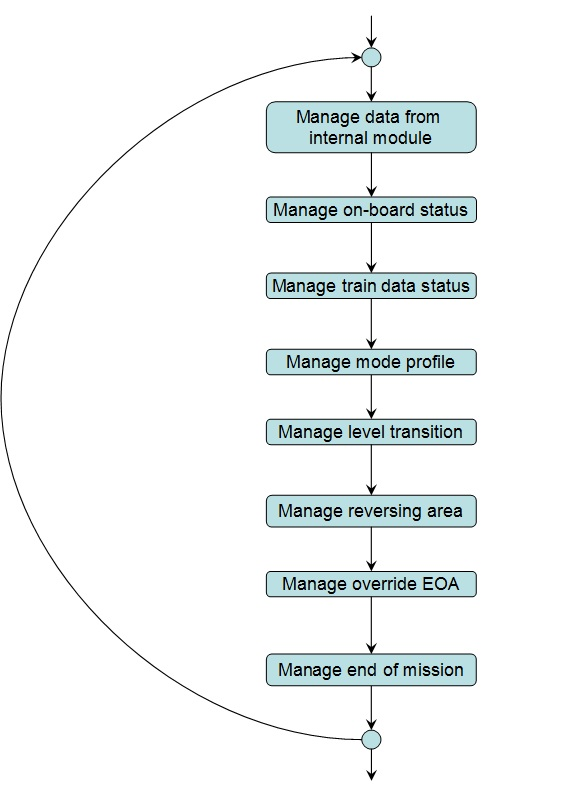
\includegraphics[width=\textwidth]{image/evc_mode_level_manager}
  \caption{Mode/level manager, sequence diagram}
  \label{fig:Mode/level manager, sequence diagram}
\end{figure}
\subsection{Manage data from internal module}
It manages the reception of data from other modules:
\begin{itemize}
\item Mode profile data: it is stored for the management of the mode profile.
\item Level transition data: it is stored for the management of the level transition.
\item Reversing area data: it is stored for the management of the reversing area.
\item Driver acknowledgement, action: it is used in the management of the on-board status.
\item Internal event (RBC answer, train trip request, ...): it is used in the management of the on-board status.
\end{itemize}

\subsection{Manage on-board status}
It manages the status of the on-board according to the current ETCS level, the received event (driver action, RBC answer, ...), the TIU data (power on/off, cabin status, ...). 
It sets the ETCS mode. 
It manages the required actions in the current status.

\subsection{Manage train data status}
It manages the status of the train data according to the mode changes and the driver data entry.

\subsection{Manage mode profile}
It manages the entry / exit in shunting or on sight according to the stored mode profile. 
It manages the acknowledgement request to the driver.

\subsection{Manage level transition}
According to the stored level transition data and the available train equipments, it selects the suitable level transition. 
It performs the level transition at the required location and sets the new level. 
It manages the acknowledgement request to the driver for the level transition. 
It manages the mode change due to the level transition if required.

\subsection{Manage reversing area}
According to the stored reversing area data, it manages the indication to the driver of the area where the selection of reversing is possible.

\subsection{Manage override EOA}
It manages the override EOA request from the driver, the inhibition of the transition to trip. 
It manages the end of the override EOA according to the National values, train trip request or former EOA.

\subsection{Manage end of mission}
It manages the end of mission procedure according to the mode change. In level 2/3, it requests the sending of end of mission radio message. 
It manages the repetition of the sending of the radio message if required. 
It requests the disconnection if no disconnection order has been received from the RBC.

\appendix
\chapter{Glossary}
			\begin{longtable}{|l|l|l|}
				\caption{Glossary}\\ 
				\hline
				
					\begin{minipage}[t]{0.40\linewidth} \textbf{Term}	\end{minipage} 
				&	\begin{minipage}[t]{0.20\linewidth} \textbf{Abb.}	\end{minipage} 
				&	\begin{minipage}[t]{0.40\linewidth} \textbf{Description} \end{minipage} \\
				
				\hline
					\begin{minipage}[t]{0.40\linewidth} European Vital Computer	\end{minipage} 
				&	\begin{minipage}[t]{0.20\linewidth} EVC	\end{minipage} 
				&	\begin{minipage}[t]{0.40\linewidth} \end{minipage} \\
				
				\hline
					\begin{minipage}[t]{0.40\linewidth} Train Interface Unit	\end{minipage} 
				&	\begin{minipage}[t]{0.20\linewidth} TIU	\end{minipage} 
				&	\begin{minipage}[t]{0.40\linewidth} \end{minipage} \\
				
				\hline
					\begin{minipage}[t]{0.40\linewidth} Driver Machine Interface	\end{minipage} 
				&	\begin{minipage}[t]{0.20\linewidth} DMI	\end{minipage} 
				&	\begin{minipage}[t]{0.40\linewidth} \end{minipage} \\
				
				\hline
					\begin{minipage}[t]{0.40\linewidth} Juridical Recording Unit	\end{minipage} 
				&	\begin{minipage}[t]{0.20\linewidth} JRU	\end{minipage} 
				&	\begin{minipage}[t]{0.40\linewidth}  \end{minipage} \\
				
				\hline
					\begin{minipage}[t]{0.40\linewidth} Graphical User Interface	\end{minipage} 
				&	\begin{minipage}[t]{0.20\linewidth} GUI	\end{minipage} 
				&	\begin{minipage}[t]{0.40\linewidth}\end{minipage} \\
				
				\hline
					\begin{minipage}[t]{0.40\linewidth} Kilometer Point	\end{minipage} 
				&	\begin{minipage}[t]{0.20\linewidth} KP\end{minipage} 
				&	\begin{minipage}[t]{0.40\linewidth}\end{minipage} \\
				
				\hline
					\begin{minipage}[t]{0.40\linewidth} Radio Block Centre	\end{minipage} 
				&	\begin{minipage}[t]{0.20\linewidth} RBC\end{minipage} 
				&	\begin{minipage}[t]{0.40\linewidth}\end{minipage} \\
				
				\hline
				\begin{minipage}[t]{0.40\linewidth} Radio Infill Unit	\end{minipage} 
				&	\begin{minipage}[t]{0.20\linewidth} RIU\end{minipage} 
				&	\begin{minipage}[t]{0.40\linewidth}\end{minipage} \\
				
				\hline
				\begin{minipage}[t]{0.40\linewidth} Radio Interface Module	\end{minipage} 
				&	\begin{minipage}[t]{0.20\linewidth} RIM\end{minipage} 
				&	\begin{minipage}[t]{0.40\linewidth}\end{minipage} \\
				
				\hline
				\begin{minipage}[t]{0.40\linewidth} Movement authority	\end{minipage} 
				&	\begin{minipage}[t]{0.20\linewidth} MA\end{minipage} 
				&	\begin{minipage}[t]{0.40\linewidth}\end{minipage} \\
				
				\hline
				
																																								
			\end{longtable}	
\chapter{Odometric data}
\label{odometric_data}
The following data are received from the odometer:
\newline
\newline
			\begin{longtable}{|l|l|l|}
				\caption{Odometric data}\\ 
				\hline
				
					\begin{minipage}[t]{0.20\linewidth} \textbf{Name}	\end{minipage} 
				&	\begin{minipage}[t]{0.10\linewidth} \textbf{Unit}	\end{minipage} 
				&	\begin{minipage}[t]{0.70\linewidth} \textbf{Description} \end{minipage} \\
				
				\hline
				\begin{minipage}[t]{0.20\linewidth} Position	\end{minipage} 
				&	\begin{minipage}[t]{0.10\linewidth} $m$\end{minipage} 
				&	\begin{minipage}[t]{0.70\linewidth}Absolute train location\end{minipage} \\
				
				\hline
				\begin{minipage}[t]{0.20\linewidth} Speed	\end{minipage} 
				&	\begin{minipage}[t]{0.10\linewidth} $m/s$\end{minipage} 
				&	\begin{minipage}[t]{0.70\linewidth}Train speed.
				\newline
				If it has a positive value, the train is moving forward, otherwise it is moving backward.
				\end{minipage} \\
								
				\hline
				\begin{minipage}[t]{0.20\linewidth} Acceleration	\end{minipage} 
				&	\begin{minipage}[t]{0.10\linewidth} $m/s^2$\end{minipage} 
				&	\begin{minipage}[t]{0.70\linewidth}Train acceleration.
				\newline
				If it has a positive value, the train accelerates (the absolute value of the train speed increases), otherwise the train decelerates (the absolute value of the train speed decreases).
				\end{minipage} \\
								
				\hline
																																	
			\end{longtable}	
\chapter{TIU data}
\label{tiu_data}
The following data are received from the TIU:
			\begin{longtable}{|l|l|}
				\caption{TIU received data}\\ 
				\hline
					\begin{minipage}[t]{0.5\linewidth} \textbf{Name}	\end{minipage} 
				&	\begin{minipage}[t]{0.5\linewidth} \textbf{Range} \end{minipage} \\
				
				\hline
					\begin{minipage}[t]{0.5\linewidth} Main power switch status	\end{minipage} 
				&	\begin{minipage}[t]{0.5\linewidth}
						\begin{itemize}
							\item 0: power off
							\item 1: power on
						\end{itemize}
					\end{minipage} \\
					
				\hline
				\begin{minipage}[t]{0.5\linewidth} Train integrity status	\end{minipage} 
				&	\begin{minipage}[t]{0.5\linewidth}
						\begin{itemize}
							\item 0: train integrity lost
							\item 1: train integrity
						\end{itemize}
					\end{minipage} \\
				\hline
				\begin{minipage}[t]{0.5\linewidth} Sleeping permission\end{minipage} 
				&	\begin{minipage}[t]{0.5\linewidth}
						\begin{itemize}
							\item 0: no sleeping signal
							\item 1: sleeping signal is set
						\end{itemize}
					\end{minipage} \\

				\hline
				\begin{minipage}[t]{0.5\linewidth} Non leading permission\end{minipage} 
				&	\begin{minipage}[t]{0.5\linewidth}
						\begin{itemize}
							\item 0: no leading signal
							\item 1: leading signal is set
						\end{itemize}
					\end{minipage} \\
				\hline
				\begin{minipage}[t]{0.5\linewidth} Passive shunting permission\end{minipage} 
				&	\begin{minipage}[t]{0.5\linewidth}
						\begin{itemize}
							\item 0: no passive shunting signal
							\item 1: passive shunting signal is set
						\end{itemize}
					\end{minipage} \\
				\hline
				\begin{minipage}[t]{0.5\linewidth} Active cabin status	\end{minipage} 
				&	\begin{minipage}[t]{0.5\linewidth}
						\begin{itemize}
							\item 0: all cabins are closed
							\item 1: cabin A is open
							\item 2: cabin B is open
							\item 3: cabin A \& B are open
						\end{itemize}
					\end{minipage} \\
				\hline
				\begin{minipage}[t]{0.5\linewidth} Direction controller position	\end{minipage} 
				&	\begin{minipage}[t]{0.5\linewidth}
						\begin{itemize}
							\item 0: forward direction
							\item 1: backward direction
							\item 2: neutral position
						\end{itemize}
					\end{minipage} \\
				\hline
				\begin{minipage}[t]{0.5\linewidth} Regenerative brake status	\end{minipage} 
				&	\begin{minipage}[t]{0.5\linewidth}
						\begin{itemize}
							\item 0: regenerative brakes are not applied
							\item 1: regenerative brakes are applied
						\end{itemize}
					\end{minipage} \\
				\hline
				\begin{minipage}[t]{0.5\linewidth} Magnetic shoe brake status	\end{minipage} 
				&	\begin{minipage}[t]{0.5\linewidth}
						\begin{itemize}
							\item 0: magnetic shoe brakes are not applied
							\item 1: magnetic shoe brakes are applied
						\end{itemize}
					\end{minipage} \\
				\hline
				\begin{minipage}[t]{0.5\linewidth} Eddy current brake status	\end{minipage} 
				&	\begin{minipage}[t]{0.5\linewidth}
						\begin{itemize}
							\item 0: eddy current brakes are not applied
							\item 1: eddy current brakes are applied
						\end{itemize}
					\end{minipage} \\
				\hline
				\begin{minipage}[t]{0.5\linewidth} Regenerative brake status	\end{minipage} 
				&	\begin{minipage}[t]{0.5\linewidth}
						\begin{itemize}
							\item 0: electro pneumatic brakes are not applied
							\item 1: electro pneumatic brakes are applied
						\end{itemize}
					\end{minipage} \\
				\hline
				\begin{minipage}[t]{0.5\linewidth} Additional brake status	\end{minipage} 
				&	\begin{minipage}[t]{0.5\linewidth}
						\begin{itemize}
							\item 0: additional brakes are not applied
							\item 1: additional brakes are applied
						\end{itemize}
					\end{minipage} \\					
				\hline
				\begin{minipage}[t]{0.5\linewidth} Traction status	\end{minipage} 
					&	\begin{minipage}[t]{0.5\linewidth}
							\begin{itemize}
								\item 0: no traction
								\item 1: traction is set
							\end{itemize}
						\end{minipage} \\					
					\hline
				\begin{minipage}[t]{0.5\linewidth} National system isolation status	\end{minipage} 
				&	\begin{minipage}[t]{0.5\linewidth}
						\begin{itemize}
							\item 0: no national system isolation
							\item 1: national system isolation is set
						\end{itemize}
					\end{minipage} \\
				\hline
				\begin{minipage}[t]{0.5\linewidth} Brake pressure	\end{minipage} 
				&	\begin{minipage}[t]{0.5\linewidth}
						\begin{itemize}
							\item 0.0 bar to 5.0 bar
						\end{itemize}
					\end{minipage} \\
				\hline
				\begin{minipage}[t]{0.5\linewidth} Train data information	\end{minipage} 
				&	\begin{minipage}[t]{0.5\linewidth}
					\end{minipage} \\					
				\hline
				\begin{minipage}[t]{0.5\linewidth} Type of train data entry	\end{minipage} 
				&	\begin{minipage}[t]{0.5\linewidth}
					\end{minipage} \\					
				\hline
			\end{longtable}
				
The following data are sent to the TIU:	
			\begin{longtable}{|l|l|}
				\caption{TIU sent data}\\ 
				\hline
				
					\begin{minipage}[t]{0.5\linewidth} \textbf{Name}	\end{minipage} 
				&	\begin{minipage}[t]{0.5\linewidth} \textbf{Range} \end{minipage} \\
				\hline
					\begin{minipage}[t]{0.5\linewidth}Traction cut off request	\end{minipage} 
				&	\begin{minipage}[t]{0.5\linewidth}
						\begin{itemize}
							\item 0: no request for traction cut off
							\item 1: request for traction cut off
						\end{itemize}
					\end{minipage} \\
				\hline
				\begin{minipage}[t]{0.5\linewidth} Service brakes application request	\end{minipage} 
				&	\begin{minipage}[t]{0.5\linewidth}
						\begin{itemize}
							\item 0: no request for service brakes application
							\item 1: request for service brakes application
						\end{itemize}
					\end{minipage} \\
				\hline
				
				\begin{minipage}[t]{0.5\linewidth} Emergency brakes application request	\end{minipage} 
				&	\begin{minipage}[t]{0.5\linewidth}
						\begin{itemize}
							\item 0: no request for emergency brakes application
							\item 1: request for emergency brakes application
						\end{itemize}
					\end{minipage} \\
				\hline
				\begin{minipage}[t]{0.5\linewidth} Inhibition of regenerative brakes request	\end{minipage} 
				&	\begin{minipage}[t]{0.5\linewidth}
						\begin{itemize}
							\item 0: no request to inhibit the regenerative brakes
							\item 1: request to inhibit the regenerative brakes
						\end{itemize}
					\end{minipage} \\
				\hline
				\begin{minipage}[t]{0.5\linewidth} Inhibition of magnetic shoe brakes request	\end{minipage} 
				&	\begin{minipage}[t]{0.5\linewidth}
						\begin{itemize}
							\item 0: no request to inhibit the magnetic shoe brakes
							\item 1: request to inhibit the magnetic shoe brakes
						\end{itemize}
					\end{minipage} \\
				\hline
				\begin{minipage}[t]{0.5\linewidth} Inhibition of eddy current brakes for SB request	\end{minipage} 
				&	\begin{minipage}[t]{0.5\linewidth}
						\begin{itemize}
							\item 0: no request to inhibit the eddy current brakes for SB
							\item 1: request to inhibit the eddy current brakes for SB
						\end{itemize}
					\end{minipage} \\
				\hline
				\begin{minipage}[t]{0.5\linewidth} Inhibition of eddy current brakes for EB request	\end{minipage} 
				&	\begin{minipage}[t]{0.5\linewidth}
						\begin{itemize}
							\item 0: no request to inhibit the eddy current brakes for EB
							\item 1: request to inhibit the eddy current brakes for EB
						\end{itemize}
					\end{minipage} \\
				\hline				
				\begin{minipage}[t]{0.5\linewidth} Main circuit breaker open request	\end{minipage} 
				&	\begin{minipage}[t]{0.5\linewidth}
						\begin{itemize}
							\item 0: no request to open main circuit breaker
							\item 1: request to open main circuit breaker
						\end{itemize}
					\end{minipage} \\
				\hline
				
				\begin{minipage}[t]{0.5\linewidth} Pantograph request	\end{minipage} 
				&	\begin{minipage}[t]{0.5\linewidth}
						\begin{itemize}
							\item 0: request for pantograph low
							\item 1: request for pantograph down
						\end{itemize}
					\end{minipage} \\
				\hline
				\begin{minipage}[t]{0.5\linewidth} Airtight request	\end{minipage} 
				&	\begin{minipage}[t]{0.5\linewidth}
						\begin{itemize}
							\item 0: no request for airtight
							\item 1: request for airtight
						\end{itemize}
					\end{minipage} \\
				\hline
				\begin{minipage}[t]{0.5\linewidth} Isolation status	\end{minipage} 
				&	\begin{minipage}[t]{0.5\linewidth}
						\begin{itemize}
							\item 0: no isolation
							\item 1: isolation is set
						\end{itemize}
					\end{minipage} \\
				\hline
				\begin{minipage}[t]{0.5\linewidth} Change of traction system	\end{minipage} 
				&	\begin{minipage}[t]{0.5\linewidth}
						\begin{itemize}
							\item 600V DC to 25 kV AC
						\end{itemize}
					\end{minipage} \\
				\hline
				\begin{minipage}[t]{0.5\linewidth} Status location	\end{minipage} 
				&	\begin{minipage}[t]{0.5\linewidth}
					\end{minipage} \\
				\hline
				\begin{minipage}[t]{0.5\linewidth} Allowed current consumption	\end{minipage} 
				&	\begin{minipage}[t]{0.5\linewidth}
						\begin{itemize}
							\item 0 A to 10000 A
						\end{itemize}
					\end{minipage} \\
				\hline				
				\end{longtable}
\chapter{EuroRadio data}
\label{euroradio_data}
The communication between the EVC and the EuroRadio is based on the exchanged of radio primitives.
The following primitives are available:
			\begin{longtable}{|l|l|l|}
				\caption{Connection on EVC initiative}\\ 
				\hline
				
					\begin{minipage}[t]{0.3\linewidth} \textbf{Primitive}	\end{minipage}
				&	\begin{minipage}[t]{0.6\linewidth} \textbf{Description}	\end{minipage}
				&	\begin{minipage}[t]{0.1\linewidth} \textbf{Dir.} \end{minipage} \\
				
				\hline
				
					\begin{minipage}[t]{0.3\linewidth}Connection request \end{minipage}
					&\begin{minipage}[t]{0.6\linewidth} This primitive is used to request a connection establishment.	\end{minipage}
					&\begin{minipage}[t]{0.1\linewidth} $\Rightarrow$  \end{minipage} \\
				
				\hline
								
					\begin{minipage}[t]{0.3\linewidth}Connection confirm \end{minipage}
					&\begin{minipage}[t]{0.6\linewidth} This primitive is used to confirm a connection establishment after a request.	\end{minipage}
					&\begin{minipage}[t]{0.1\linewidth} $\Leftarrow$ \end{minipage} \\
				
				\hline									
			\end{longtable}
			
			\begin{longtable}{|l|l|l|}
				\caption{Connection on RBC initiative}\\ 
				\hline
				
					\begin{minipage}[t]{0.3\linewidth} \textbf{Primitive}	\end{minipage}
				&	\begin{minipage}[t]{0.6\linewidth} \textbf{Description}	\end{minipage}
				&	\begin{minipage}[t]{0.1\linewidth} \textbf{Dir.} \end{minipage} \\
				
				\hline
				
					\begin{minipage}[t]{0.3\linewidth}Connection indication \end{minipage}
					&\begin{minipage}[t]{0.6\linewidth} This primitive is used to indicate a connection establishment.	\end{minipage}
					&\begin{minipage}[t]{0.1\linewidth} $\Rightarrow$ \end{minipage} \\
				
				\hline
								
					\begin{minipage}[t]{0.3\linewidth}Connection response \end{minipage}
					&\begin{minipage}[t]{0.6\linewidth} This primitive is used to respond to a connection establishment indication.	\end{minipage}
					&\begin{minipage}[t]{0.1\linewidth} $\Leftarrow$ \end{minipage} \\
				
				\hline									
			\end{longtable}
						
			\begin{longtable}{|l|l|l|}
				\caption{Transmission of data}\\ 
				\hline
				
					\begin{minipage}[t]{0.3\linewidth} \textbf{Primitive}	\end{minipage}
				&	\begin{minipage}[t]{0.6\linewidth} \textbf{Description}	\end{minipage}
				&	\begin{minipage}[t]{0.1\linewidth} \textbf{Dir.} \end{minipage} \\
				
				\hline
				
					\begin{minipage}[t]{0.3\linewidth}Data request \end{minipage}
					&\begin{minipage}[t]{0.6\linewidth} This primitive is used to request the transmission of a radio message.	\end{minipage}
					&\begin{minipage}[t]{0.1\linewidth} $\Rightarrow$ \end{minipage} \\
				
				\hline
								
					\begin{minipage}[t]{0.3\linewidth}Data indication \end{minipage}
					&\begin{minipage}[t]{0.6\linewidth} This primitive is used to indicate the reception of a radio message.\end{minipage}
					&\begin{minipage}[t]{0.1\linewidth} $\Leftarrow$ \end{minipage} \\
				
				\hline
													
				\begin{minipage}[t]{0.3\linewidth}High priority data request \end{minipage}
					&\begin{minipage}[t]{0.6\linewidth} This primitive is used to request the transmission of an emergency radio message.	\end{minipage}
					&\begin{minipage}[t]{0.1\linewidth} $\Rightarrow$ \end{minipage} \\
				
				\hline	
													
				\begin{minipage}[t]{0.3\linewidth}High priority data indication \end{minipage}
					&\begin{minipage}[t]{0.6\linewidth} This primitive is used to indicate the reception of an emergency radio message.	\end{minipage}
					&\begin{minipage}[t]{0.1\linewidth} $\Leftarrow$ \end{minipage} \\
				
				\hline										
			\end{longtable}		
					
					
			\begin{longtable}{|l|l|l|}
				\caption{Disconnection}\\ 
				\hline
				
					\begin{minipage}[t]{0.3\linewidth} \textbf{Primitive}	\end{minipage}
				&	\begin{minipage}[t]{0.6\linewidth} \textbf{Description}	\end{minipage}
				&	\begin{minipage}[t]{0.1\linewidth} \textbf{Dir.} \end{minipage} \\
				
				\hline
				
					\begin{minipage}[t]{0.3\linewidth}Disconnection request \end{minipage}
					&\begin{minipage}[t]{0.6\linewidth} This primitive is used to request a disconnection.	\end{minipage}
					&\begin{minipage}[t]{0.1\linewidth} $\Rightarrow$ \end{minipage} \\
				
				\hline
								
					\begin{minipage}[t]{0.3\linewidth}Disconnection indication \end{minipage}
					&\begin{minipage}[t]{0.6\linewidth} This primitive is used to indicate a disconnection (after a request or due to other reason).	\end{minipage}
					&\begin{minipage}[t]{0.1\linewidth} $\Leftarrow$ \end{minipage} \\
				
				\hline									
			\end{longtable}					
						
\section{Format of the exchanged primitives}
The primitives are exchanged between the EVC simulator and the EuroRadio according to the following format:
			\begin{longtable}{|l|l|l|}
				\caption{Format of the exchanged primitives}\\ 
				\hline
				
					\begin{minipage}[t]{0.2\linewidth} \textbf{Size}	\end{minipage}
				&	\begin{minipage}[t]{0.6\linewidth} \textbf{Description}	\end{minipage}
				&	\begin{minipage}[t]{0.2\linewidth} \textbf{Range} \end{minipage} \\
				
				\hline
				
					\begin{minipage}[t]{0.2\linewidth}2 bytes \end{minipage}
					&\begin{minipage}[t]{0.6\linewidth} Length of the radio primitive (in bytes)	\end{minipage}
					&\begin{minipage}[t]{0.2\linewidth} \end{minipage} \\
				
				\hline
								
					\begin{minipage}[t]{0.2\linewidth}1 byte \end{minipage}
					&\begin{minipage}[t]{0.6\linewidth} Identity of the radio primitive.	\end{minipage}
					&\begin{minipage}[t]{0.2\linewidth} \end{minipage} \\
				
				\hline

					\begin{minipage}[t]{0.2\linewidth}n bytes \end{minipage}
					&\begin{minipage}[t]{0.6\linewidth} Content of the message according to the radio primitive identity.	\end{minipage}
					&\begin{minipage}[t]{0.2\linewidth} \end{minipage} \\
				
				\hline														
			\end{longtable}
\subsection{Connection request}
This primitive is used to request a connection (EVC $\rightarrow$ EuroRadio).
			\begin{longtable}{|l|l|l|}
				\caption{Connection request}\\ 
				\hline
				
					\begin{minipage}[t]{0.1\linewidth} \textbf{Size}	\end{minipage}
				&	\begin{minipage}[t]{0.5\linewidth} \textbf{Description}	\end{minipage}
				&	\begin{minipage}[t]{0.3\linewidth} \textbf{Range} \end{minipage} \\
				
				\hline
					 \begin{minipage}[t]{0.1\linewidth}1 byte \end{minipage}
					&\begin{minipage}[t]{0.6\linewidth}Identity of the radio primitive "`Connection request"'	\end{minipage}
					&\begin{minipage}[t]{0.3\linewidth}0x01 (fixed) \end{minipage} \\
				
				\hline
					\begin{minipage}[t]{0.1\linewidth}1 byte \end{minipage}
					&\begin{minipage}[t]{0.6\linewidth} Address type 	\end{minipage}
					&\begin{minipage}[t]{0.3\linewidth}0x01 (fixed) \end{minipage} \\
				
				\hline
					\begin{minipage}[t]{0.1\linewidth}1 byte \end{minipage}
					&\begin{minipage}[t]{0.6\linewidth} Size of called number (in bytes)	\end{minipage}
					&\begin{minipage}[t]{0.3\linewidth}0 to 16 \end{minipage} \\
				
				\hline
					\begin{minipage}[t]{0.1\linewidth}1 byte \end{minipage}
					&\begin{minipage}[t]{0.6\linewidth} Reserved	\end{minipage}
					&\begin{minipage}[t]{0.3\linewidth}0x00 (fixed) \end{minipage} \\
				
				\hline
					\begin{minipage}[t]{0.1\linewidth}16 bytes \end{minipage}
					&\begin{minipage}[t]{0.6\linewidth} Called number (the unused bytes are coded as 0x00)	\end{minipage}
					&\begin{minipage}[t]{0.3\linewidth} \end{minipage} \\
				
				\hline
					\begin{minipage}[t]{0.1\linewidth}1 byte \end{minipage}
					&\begin{minipage}[t]{0.6\linewidth} Called ETCS Id type	\end{minipage}
					&\begin{minipage}[t]{0.3\linewidth}
						\begin{itemize}
							\item 0x01: RBC/RIU
							\item 0x02: train
						\end{itemize}
					\end{minipage} \\
				
				\hline
					\begin{minipage}[t]{0.1\linewidth}3 bytes \end{minipage}
					&\begin{minipage}[t]{0.6\linewidth} Called ETCS Id (NID\_ENGINE or NID\_RBC)	\end{minipage}
					&\begin{minipage}[t]{0.3\linewidth} \end{minipage} \\
				
				\hline
					\begin{minipage}[t]{0.1\linewidth}1 byte \end{minipage}
					&\begin{minipage}[t]{0.6\linewidth} Calling ETCS Id type\end{minipage}
					&\begin{minipage}[t]{0.3\linewidth}
						\begin{itemize}
							\item 0x01: RBC/RIU
							\item 0x02: train
						\end{itemize}
					\end{minipage} \\
				
				\hline
					\begin{minipage}[t]{0.1\linewidth}3 bytes \end{minipage}
					&\begin{minipage}[t]{0.6\linewidth} Calling ETCS Id (NID\_ENGINE or NID\_RBC )	\end{minipage}
					&\begin{minipage}[t]{0.3\linewidth} \end{minipage} \\
				
				\hline
					\begin{minipage}[t]{0.1\linewidth}1 byte \end{minipage}
					&\begin{minipage}[t]{0.6\linewidth} Application type (fixed)	\end{minipage}
					&\begin{minipage}[t]{0.3\linewidth}0x10 (fixed) \end{minipage} \\
				
				\hline
					\begin{minipage}[t]{0.1\linewidth}2 bytes \end{minipage}
					&\begin{minipage}[t]{0.6\linewidth} Quality of service	\end{minipage}
					&\begin{minipage}[t]{0.3\linewidth} \end{minipage} \\
				
				\hline
			\end{longtable}
			Length: 31 bytes
\subsection{Connection indication}
This primitive is used to indicate that a safe connection is established (EuroRadio $\rightarrow$ EVC).
			\begin{longtable}{|l|l|l|}
				\caption{Connection indication}\\ 
				\hline
				
					\begin{minipage}[t]{0.1\linewidth} \textbf{Size}	\end{minipage}
				&	\begin{minipage}[t]{0.5\linewidth} \textbf{Description}	\end{minipage}
				&	\begin{minipage}[t]{0.3\linewidth} \textbf{Range} \end{minipage} \\
				
				\hline
					 \begin{minipage}[t]{0.1\linewidth}1 byte \end{minipage}
					&\begin{minipage}[t]{0.6\linewidth}Identity of the radio primitive "`Connection indication"'	\end{minipage}
					&\begin{minipage}[t]{0.3\linewidth}0x03 (fixed) \end{minipage} \\
					
				\hline
					 \begin{minipage}[t]{0.1\linewidth}4 bytes \end{minipage}
					&\begin{minipage}[t]{0.6\linewidth}Connection identifier (SaCEPID)	\end{minipage}
					&\begin{minipage}[t]{0.3\linewidth}\end{minipage} \\
					
				\hline
					 \begin{minipage}[t]{0.1\linewidth}1 byte \end{minipage}
					&\begin{minipage}[t]{0.6\linewidth}Called ETCS Id type\end{minipage}
					&\begin{minipage}[t]{0.3\linewidth}
						\begin{itemize}
							\item 0x01: RBC/RIU
							\item 0x02: train
						\end{itemize}
					\end{minipage} \\
					
				\hline
					 \begin{minipage}[t]{0.1\linewidth}3 bytes \end{minipage}
					&\begin{minipage}[t]{0.6\linewidth}Called ETCS Id (NID\_ENGINE or NID\_RBC )\end{minipage}
					&\begin{minipage}[t]{0.3\linewidth}\end{minipage} \\
					
				\hline
					 \begin{minipage}[t]{0.1\linewidth}1 byte \end{minipage}
					&\begin{minipage}[t]{0.6\linewidth}Calling ETCS Id type	\end{minipage}
					&\begin{minipage}[t]{0.3\linewidth}
						\begin{itemize}
							\item 0x01: RBC/RIU
							\item 0x02: train
						\end{itemize}
					\end{minipage} \\
					
				\hline
					 \begin{minipage}[t]{0.1\linewidth}3 bytes \end{minipage}
					&\begin{minipage}[t]{0.6\linewidth}Calling ETCS Id (NID\_ENGINE or NID\_RBC )	\end{minipage}
					&\begin{minipage}[t]{0.3\linewidth}\end{minipage} \\
					
				\hline
					 \begin{minipage}[t]{0.1\linewidth}1 byte \end{minipage}
					&\begin{minipage}[t]{0.6\linewidth}Application type \end{minipage}
					&\begin{minipage}[t]{0.3\linewidth}0x10 (fixed) \end{minipage} \\
					
				\hline
					 \begin{minipage}[t]{0.1\linewidth}2 bytes \end{minipage}
					&\begin{minipage}[t]{0.6\linewidth}Quality of service\end{minipage}
					&\begin{minipage}[t]{0.3\linewidth}\end{minipage} \\
				
				\hline
			\end{longtable}
			Length: 16 bytes
\subsection{Connection response}
This primitive is used to respond on reception of "`connection indication"' (EVC $\rightarrow$ EuroRadio).
			\begin{longtable}{|l|l|l|}
				\caption{Connection response}\\ 
				\hline
				
					\begin{minipage}[t]{0.1\linewidth} \textbf{Size}	\end{minipage}
				&	\begin{minipage}[t]{0.5\linewidth} \textbf{Description}	\end{minipage}
				&	\begin{minipage}[t]{0.3\linewidth} \textbf{Range} \end{minipage} \\
				
				\hline
					 \begin{minipage}[t]{0.1\linewidth}1 byte \end{minipage}
					&\begin{minipage}[t]{0.6\linewidth}Identity of the radio primitive "`Connection response"'	\end{minipage}
					&\begin{minipage}[t]{0.3\linewidth}0x02 (fixed) \end{minipage} \\
					
				\hline
					 \begin{minipage}[t]{0.1\linewidth}4 bytes \end{minipage}
					&\begin{minipage}[t]{0.6\linewidth}Connection identifier (SaCEPID)	\end{minipage}
					&\begin{minipage}[t]{0.3\linewidth} \end{minipage} \\
					
				\hline
					 \begin{minipage}[t]{0.1\linewidth}1 byte \end{minipage}
					&\begin{minipage}[t]{0.6\linewidth}Responding ETCS Id type	\end{minipage}
					&\begin{minipage}[t]{0.3\linewidth}
							\begin{itemize}
								\item 0x01: RBC/RIU
								\item 0x02: train
							\end{itemize}						
					  \end{minipage} \\
					
				\hline
					 \begin{minipage}[t]{0.1\linewidth}3 bytes \end{minipage}
					&\begin{minipage}[t]{0.6\linewidth}Responding ETCS Id (NID\_ENGINE or NID\_RBC )\end{minipage}
					&\begin{minipage}[t]{0.3\linewidth}\end{minipage} \\
				\hline
			\end{longtable}
			Length: 9 bytes
\subsection{Connection confirmation}
This primitive is used to confirm the establishment of a connection on reception of "`connection request"' (EuroRadio $\rightarrow$ EVC).
 			\begin{longtable}{|l|l|l|}
				\caption{Connection confirmation}\\ 
				\hline
				
					\begin{minipage}[t]{0.1\linewidth} \textbf{Size}	\end{minipage}
				&	\begin{minipage}[t]{0.5\linewidth} \textbf{Description}	\end{minipage}
				&	\begin{minipage}[t]{0.3\linewidth} \textbf{Range} \end{minipage} \\
				
				\hline
					 \begin{minipage}[t]{0.1\linewidth}1 byte \end{minipage}
					&\begin{minipage}[t]{0.6\linewidth}Identity of the radio primitive "`Connection confirmation"'	\end{minipage}
					&\begin{minipage}[t]{0.3\linewidth}0x04 (fixed) \end{minipage} \\
					
				\hline
					 \begin{minipage}[t]{0.1\linewidth}4 bytes \end{minipage}
					&\begin{minipage}[t]{0.6\linewidth}Connection identifier (SaCEPID)	\end{minipage}
					&\begin{minipage}[t]{0.3\linewidth} \end{minipage} \\
					
				\hline
					 \begin{minipage}[t]{0.1\linewidth}1 bytes \end{minipage}
					&\begin{minipage}[t]{0.6\linewidth}Responding ETCS Id type	\end{minipage}
					&\begin{minipage}[t]{0.3\linewidth}
							\begin{itemize}
								\item 0x01: RBC/RIU
								\item 0x02: train
							\end{itemize}						
					  \end{minipage} \\
					
				\hline
					 \begin{minipage}[t]{0.1\linewidth}3 bytes \end{minipage}
					&\begin{minipage}[t]{0.6\linewidth}Responding ETCS Id (NID\_ENGINE or NID\_RBC )\end{minipage}
					&\begin{minipage}[t]{0.3\linewidth}\end{minipage} \\
				\hline
			\end{longtable}
			Length: 9 bytes
\subsection{Data request}
This primitive is used to request the transmission of a radio message (EVC $\rightarrow$ EuroRadio).
 			\begin{longtable}{|l|l|l|}
				\caption{Data request}\\ 
				\hline
				
					\begin{minipage}[t]{0.1\linewidth} \textbf{Size}	\end{minipage}
				&	\begin{minipage}[t]{0.5\linewidth} \textbf{Description}	\end{minipage}
				&	\begin{minipage}[t]{0.3\linewidth} \textbf{Range} \end{minipage} \\
				
				\hline
					 \begin{minipage}[t]{0.1\linewidth}1 byte \end{minipage}
					&\begin{minipage}[t]{0.6\linewidth}Identity of the radio primitive "`Data request"'	\end{minipage}
					&\begin{minipage}[t]{0.3\linewidth}0x05 (fixed) \end{minipage} \\
					
				\hline
					 \begin{minipage}[t]{0.1\linewidth}4 bytes \end{minipage}
					&\begin{minipage}[t]{0.6\linewidth}Connection identifier (SaCEPID)	\end{minipage}
					&\begin{minipage}[t]{0.3\linewidth} \end{minipage} \\
					
				\hline
					 \begin{minipage}[t]{0.1\linewidth}2 bytes \end{minipage}
					&\begin{minipage}[t]{0.6\linewidth}Length of the radio message in bytes: n	\end{minipage}
					&\begin{minipage}[t]{0.3\linewidth}0 to 255 \end{minipage} \\
					
				\hline
					 \begin{minipage}[t]{0.1\linewidth}n bytes \end{minipage}
					&\begin{minipage}[t]{0.6\linewidth}Radio message according to SRS Class 1 v3.3.0 (see [/1/])	\end{minipage}
					&\begin{minipage}[t]{0.3\linewidth}\end{minipage} \\
					
				\hline	
			\end{longtable}
			Length: up to 262 bytes	
\subsection{Data indication}
This primitive is used to indicate the reception of a radio message (EuroRadio $\rightarrow$ EVC).
 			\begin{longtable}{|l|l|l|}
				\caption{Data indication}\\ 
				\hline
				
					\begin{minipage}[t]{0.1\linewidth} \textbf{Size}	\end{minipage}
				&	\begin{minipage}[t]{0.5\linewidth} \textbf{Description}	\end{minipage}
				&	\begin{minipage}[t]{0.3\linewidth} \textbf{Range} \end{minipage} \\
				
				\hline
					 \begin{minipage}[t]{0.1\linewidth}1 byte \end{minipage}
					&\begin{minipage}[t]{0.6\linewidth}Identity of the radio primitive "`Data indication"'	\end{minipage}
					&\begin{minipage}[t]{0.3\linewidth}0x06 (fixed) \end{minipage} \\
					
				\hline
					 \begin{minipage}[t]{0.1\linewidth}4 bytes \end{minipage}
					&\begin{minipage}[t]{0.6\linewidth}Connection identifier (SaCEPID)	\end{minipage}
					&\begin{minipage}[t]{0.3\linewidth} \end{minipage} \\
					
				\hline
					 \begin{minipage}[t]{0.1\linewidth}2 bytes \end{minipage}
					&\begin{minipage}[t]{0.6\linewidth}Length of the radio message in bytes: n	\end{minipage}
					&\begin{minipage}[t]{0.3\linewidth}0 to 255 \end{minipage} \\
					
				\hline
					 \begin{minipage}[t]{0.1\linewidth}n bytes \end{minipage}
					&\begin{minipage}[t]{0.6\linewidth}Radio message according to SRS Class 1 v3.3.0 (see [/1/])	\end{minipage}
					&\begin{minipage}[t]{0.3\linewidth}\end{minipage} \\
					
				\hline	
			\end{longtable}
			Length: up to 262 bytes
\subsection{Hight priority data request}
This primitive is used to request the transmission of an emergency radio message (EVC $\rightarrow$ EuroRadio).
 			\begin{longtable}{|l|l|l|}
				\caption{Hight priority data request}\\ 
				\hline
				
					\begin{minipage}[t]{0.1\linewidth} \textbf{Size}	\end{minipage}
				&	\begin{minipage}[t]{0.5\linewidth} \textbf{Description}	\end{minipage}
				&	\begin{minipage}[t]{0.3\linewidth} \textbf{Range} \end{minipage} \\
				
				\hline
					 \begin{minipage}[t]{0.1\linewidth}1 byte \end{minipage}
					&\begin{minipage}[t]{0.6\linewidth}Identity of the radio primitive "`High priority data request"'	\end{minipage}
					&\begin{minipage}[t]{0.3\linewidth}0x0B (fixed) \end{minipage} \\
					
				\hline
					 \begin{minipage}[t]{0.1\linewidth}4 bytes \end{minipage}
					&\begin{minipage}[t]{0.6\linewidth}Connection identifier (SaCEPID)	\end{minipage}
					&\begin{minipage}[t]{0.3\linewidth} \end{minipage} \\
					
				\hline
					 \begin{minipage}[t]{0.1\linewidth}2 bytes \end{minipage}
					&\begin{minipage}[t]{0.6\linewidth}Length of the radio message in bytes: n	\end{minipage}
					&\begin{minipage}[t]{0.3\linewidth}0 to 255 \end{minipage} \\
					
				\hline
					 \begin{minipage}[t]{0.1\linewidth}n bytes \end{minipage}
					&\begin{minipage}[t]{0.6\linewidth}Radio message according to SRS Class 1 v3.3.0 (see [/1/])	\end{minipage}
					&\begin{minipage}[t]{0.3\linewidth}\end{minipage} \\
					
				\hline	
			\end{longtable}
			Length: up to 262 bytes
\subsection{Hight priority data indication}
This primitive is used to indicate the reception of an emergency radio message (EuroRadio $\rightarrow$ EVC).
 			\begin{longtable}{|l|l|l|}
				\caption{Hight priority data indication}\\ 
				\hline
				
					\begin{minipage}[t]{0.1\linewidth} \textbf{Size}	\end{minipage}
				&	\begin{minipage}[t]{0.5\linewidth} \textbf{Description}	\end{minipage}
				&	\begin{minipage}[t]{0.3\linewidth} \textbf{Range} \end{minipage} \\
				
				\hline
					 \begin{minipage}[t]{0.1\linewidth}1 byte \end{minipage}
					&\begin{minipage}[t]{0.6\linewidth}Identity of the radio primitive "`Hight priority data indication"'	\end{minipage}
					&\begin{minipage}[t]{0.3\linewidth}0x0C (fixed) \end{minipage} \\
					
				\hline
					 \begin{minipage}[t]{0.1\linewidth}4 bytes \end{minipage}
					&\begin{minipage}[t]{0.6\linewidth}Connection identifier (SaCEPID)	\end{minipage}
					&\begin{minipage}[t]{0.3\linewidth} \end{minipage} \\
					
				\hline
					 \begin{minipage}[t]{0.1\linewidth}2 bytes \end{minipage}
					&\begin{minipage}[t]{0.6\linewidth}Length of the radio message in bytes: n	\end{minipage}
					&\begin{minipage}[t]{0.3\linewidth}0 to 255 \end{minipage} \\
					
				\hline
					 \begin{minipage}[t]{0.1\linewidth}n bytes \end{minipage}
					&\begin{minipage}[t]{0.6\linewidth}Radio message according to SRS Class 1 v3.3.0 (see [/1/])	\end{minipage}
					&\begin{minipage}[t]{0.3\linewidth}\end{minipage} \\
					
				\hline	
			\end{longtable}
			Length: up to 262 bytes
\subsection{Disconnection request}
This primitive is used to request a disconnection (EVC $\rightarrow$ EuroRadio).
 			\begin{longtable}{|l|l|l|}
				\caption{Disconnection request}\\ 
				\hline
				
					\begin{minipage}[t]{0.1\linewidth} \textbf{Size}	\end{minipage}
				&	\begin{minipage}[t]{0.5\linewidth} \textbf{Description}	\end{minipage}
				&	\begin{minipage}[t]{0.3\linewidth} \textbf{Range} \end{minipage} \\
				
				\hline
					 \begin{minipage}[t]{0.1\linewidth}1 byte \end{minipage}
					&\begin{minipage}[t]{0.6\linewidth}Identity of the radio primitive "`Disconnection request"'	\end{minipage}
					&\begin{minipage}[t]{0.3\linewidth}0x07 (fixed) \end{minipage} \\
					
				\hline
					 \begin{minipage}[t]{0.1\linewidth}4 bytes \end{minipage}
					&\begin{minipage}[t]{0.6\linewidth}Connection identifier (SaCEPID)	\end{minipage}
					&\begin{minipage}[t]{0.3\linewidth} \end{minipage} \\
					
				\hline
			\end{longtable}
			Length: 5 bytes
\subsection{Disconnection indication}
This primitive is used to indicate a disconnection (EuroRadio $\rightarrow$ EVC).
 			\begin{longtable}{|l|l|l|}
				\caption{Disconnection indication}\\ 
				\hline
				
					\begin{minipage}[t]{0.1\linewidth} \textbf{Size}	\end{minipage}
				&	\begin{minipage}[t]{0.5\linewidth} \textbf{Description}	\end{minipage}
				&	\begin{minipage}[t]{0.3\linewidth} \textbf{Range} \end{minipage} \\
				
				\hline
					 \begin{minipage}[t]{0.1\linewidth}1 byte \end{minipage}
					&\begin{minipage}[t]{0.6\linewidth}Identity of the radio primitive "`Disconnection indication"'	\end{minipage}
					&\begin{minipage}[t]{0.3\linewidth}0x08 (fixed) \end{minipage} \\
					
				\hline
					 \begin{minipage}[t]{0.1\linewidth}4 bytes \end{minipage}
					&\begin{minipage}[t]{0.6\linewidth}Connection identifier (SaCEPID)	\end{minipage}
					&\begin{minipage}[t]{0.3\linewidth} \end{minipage} \\
					
				\hline
						\begin{minipage}[t]{0.1\linewidth}1 bytes \end{minipage}
					&\begin{minipage}[t]{0.6\linewidth}Reason \end{minipage}
					&\begin{minipage}[t]{0.3\linewidth} \end{minipage} \\
					
				\hline
						\begin{minipage}[t]{0.1\linewidth}1 bytes \end{minipage}
					&\begin{minipage}[t]{0.6\linewidth}Sub-reason \end{minipage}
					&\begin{minipage}[t]{0.3\linewidth} \end{minipage} \\
					
				\hline
			\end{longtable}
			Length: 7 bytes

%===================================================
%Do NOT change anything below this line

\end{document}